%%%
%%% Annual Cognitive Science Conference
%%% Sample LaTeX Paper -- Proceedings Format
%%%

% Original : Ashwin Ram (ashwin@cc.gatech.edu)       04/01/1994
% Modified : Johanna Moore (jmoore@cs.pitt.edu)      03/17/1995
% Modified : David Noelle (noelle@ucsd.edu)          03/15/1996
% Modified : Pat Langley (langley@cs.stanford.edu)   01/26/1997
% Latex2e corrections by Ramin Charles Nakisa        01/28/1997
% Modified : Tina Eliassi-Rad (eliassi@cs.wisc.edu)  01/31/1998
% Modified : Trisha Yannuzzi (trisha@ircs.upenn.edu) 12/28/1999
% Modified : Mary Ellen Foster (M.E.Foster@ed.ac.uk) 12/11/2000
% Modified : Ken Forbus                              01/23/2004
% Modified : Eli M. Silk (esilk@pitt.edu)            05/24/2005
% Modified : Niels Taatgen (taatgen@cmu.edu)         10/24/2006
% Modified : David Noelle (dnoelle@ucmerced.edu)     11/19/2014
% Modified : Roger Levy (rplevy@mit.edu)             12/31/2018
% Modified : Stephanie Denison                       11/29/2025
% Modified : Dae Houlihan (daeda@mit.edu)            12/01/2025


%%% Change "letterpaper" in the following line to "a4paper" if you must.

\documentclass[10pt,letterpaper]{article}

\usepackage{cogsci}

\cogscifinalcopy %%% Uncomment this line for the final submission

%%% Bibliography %%%
\usepackage[
  style=apa,
  natbib=true,
  annotation=false,
  url=false,
]{biblatex}
\addbibresource{cogsci_bibliography_template.bib} %%% Specify the path to a BibLaTeX file
\setlength{\bibhang}{.125in}

\usepackage{float} %%% Roger Levy added this and changed figure/table placement to [H] for conformity to Word template, though floating tables and figures to top is still generally recommended!

% Sometimes it can be useful to turn off hyphenation for purposes such as spell checking of the resulting PDF.
% \usepackage[none]{hyphenat} %%% Uncomment to turn off hyphenation

%%% Custom packages %%%
\usepackage{graphicx}
\usepackage{booktabs}
\usepackage{caption}
\usepackage{subcaption}
\usepackage{dblfloatfix}
\usepackage{comment}
\usepackage{xcolor}
\usepackage{gb4e}
\noautomath
\renewcommand{\eachwordtwo}{\relsize{-1}} % format translation in glosses
% \renewcommand{\trans}{\vskip.15\baselineskip\relsize{-1}}
\renewcommand{\trans}{\vskip.15\baselineskip}


\definecolor{glaucous-bright}{HTML}{5B7DB1} % muted blue
\definecolor{opal-bright}{HTML}{3FA7A3}     % teal/green

\title{When Correlation means Causation: Pragmatic Factors modulate Causal Implicatures in Decision-Making Contexts }

%%% Format authors using helper functions from authblk package %%%
\author[1]{\mbox{Hening Wang (hening.wang@uni-tuebingen.de)}}
\author[2]{\mbox{Daniel Lassiter (dan.lassiter@ed.ac.uk)}}
\author[1]{\mbox{Michael Franke (michael.franke@uni-tuebingen.de)}}
\affil[1]{Department of General Linguistics, University of T\"ubingen}
\affil[2]{Linguistics and English Language, University of Edinburgh}

% Custum orders
\usepackage[dvipsnames]{xcolor}
\newcommand{\todo}[1]{\textcolor{red}{\textbf{TODO:} #1}}
\newcommand{\addref}[1]{\textcolor{blue}{\textbf{ADD REFERENCE} #1}}
\newcommand{\HW}[1]{\textcolor{glaucous-bright}{[HW: #1]}}
\newcommand{\mf}[1]{\textcolor{BrickRed}{[MF: #1]}}
\newcommand{\DL}[1]{\textcolor{red}{[DL: #1]}}


\begin{document}

\maketitle

\begin{abstract}

Correlational statements (e.g., “$X$ is associated with $Y$”) can be interpreted as conveying a causal relationship. 
Recent work suggests that such interpretations may be legitimate pragmatic inferences, especially in decision-relevant contexts. 
Here, we investigate whether causal enrichment of correlational language affect memory recall and message passing, how pragmatic features of the communicative context modulate them.
Our findings support a pragmatic account of causal enrichment of correlational language.

%In Experiment~1, participants who chose to act on a putative cause were more likely to reproduce correlational statements using explicitly causal language, especially when communicating advice to others, indicating that causal enrichment is reflected not only in immediate action but also in downstream communication. In Experiment~2, we introduce a belief-update paradigm that measures changes in willingness to intervene relative to an individually measured baseline, while manipulating pragmatic factors such as speaker goal orientation and directness of information.

\textbf{Keywords:}
causal implicature; correlational language; pragmatic inference; decision making; belief updating

\end{abstract}

\begin{figure*}[!t]
    \centering
    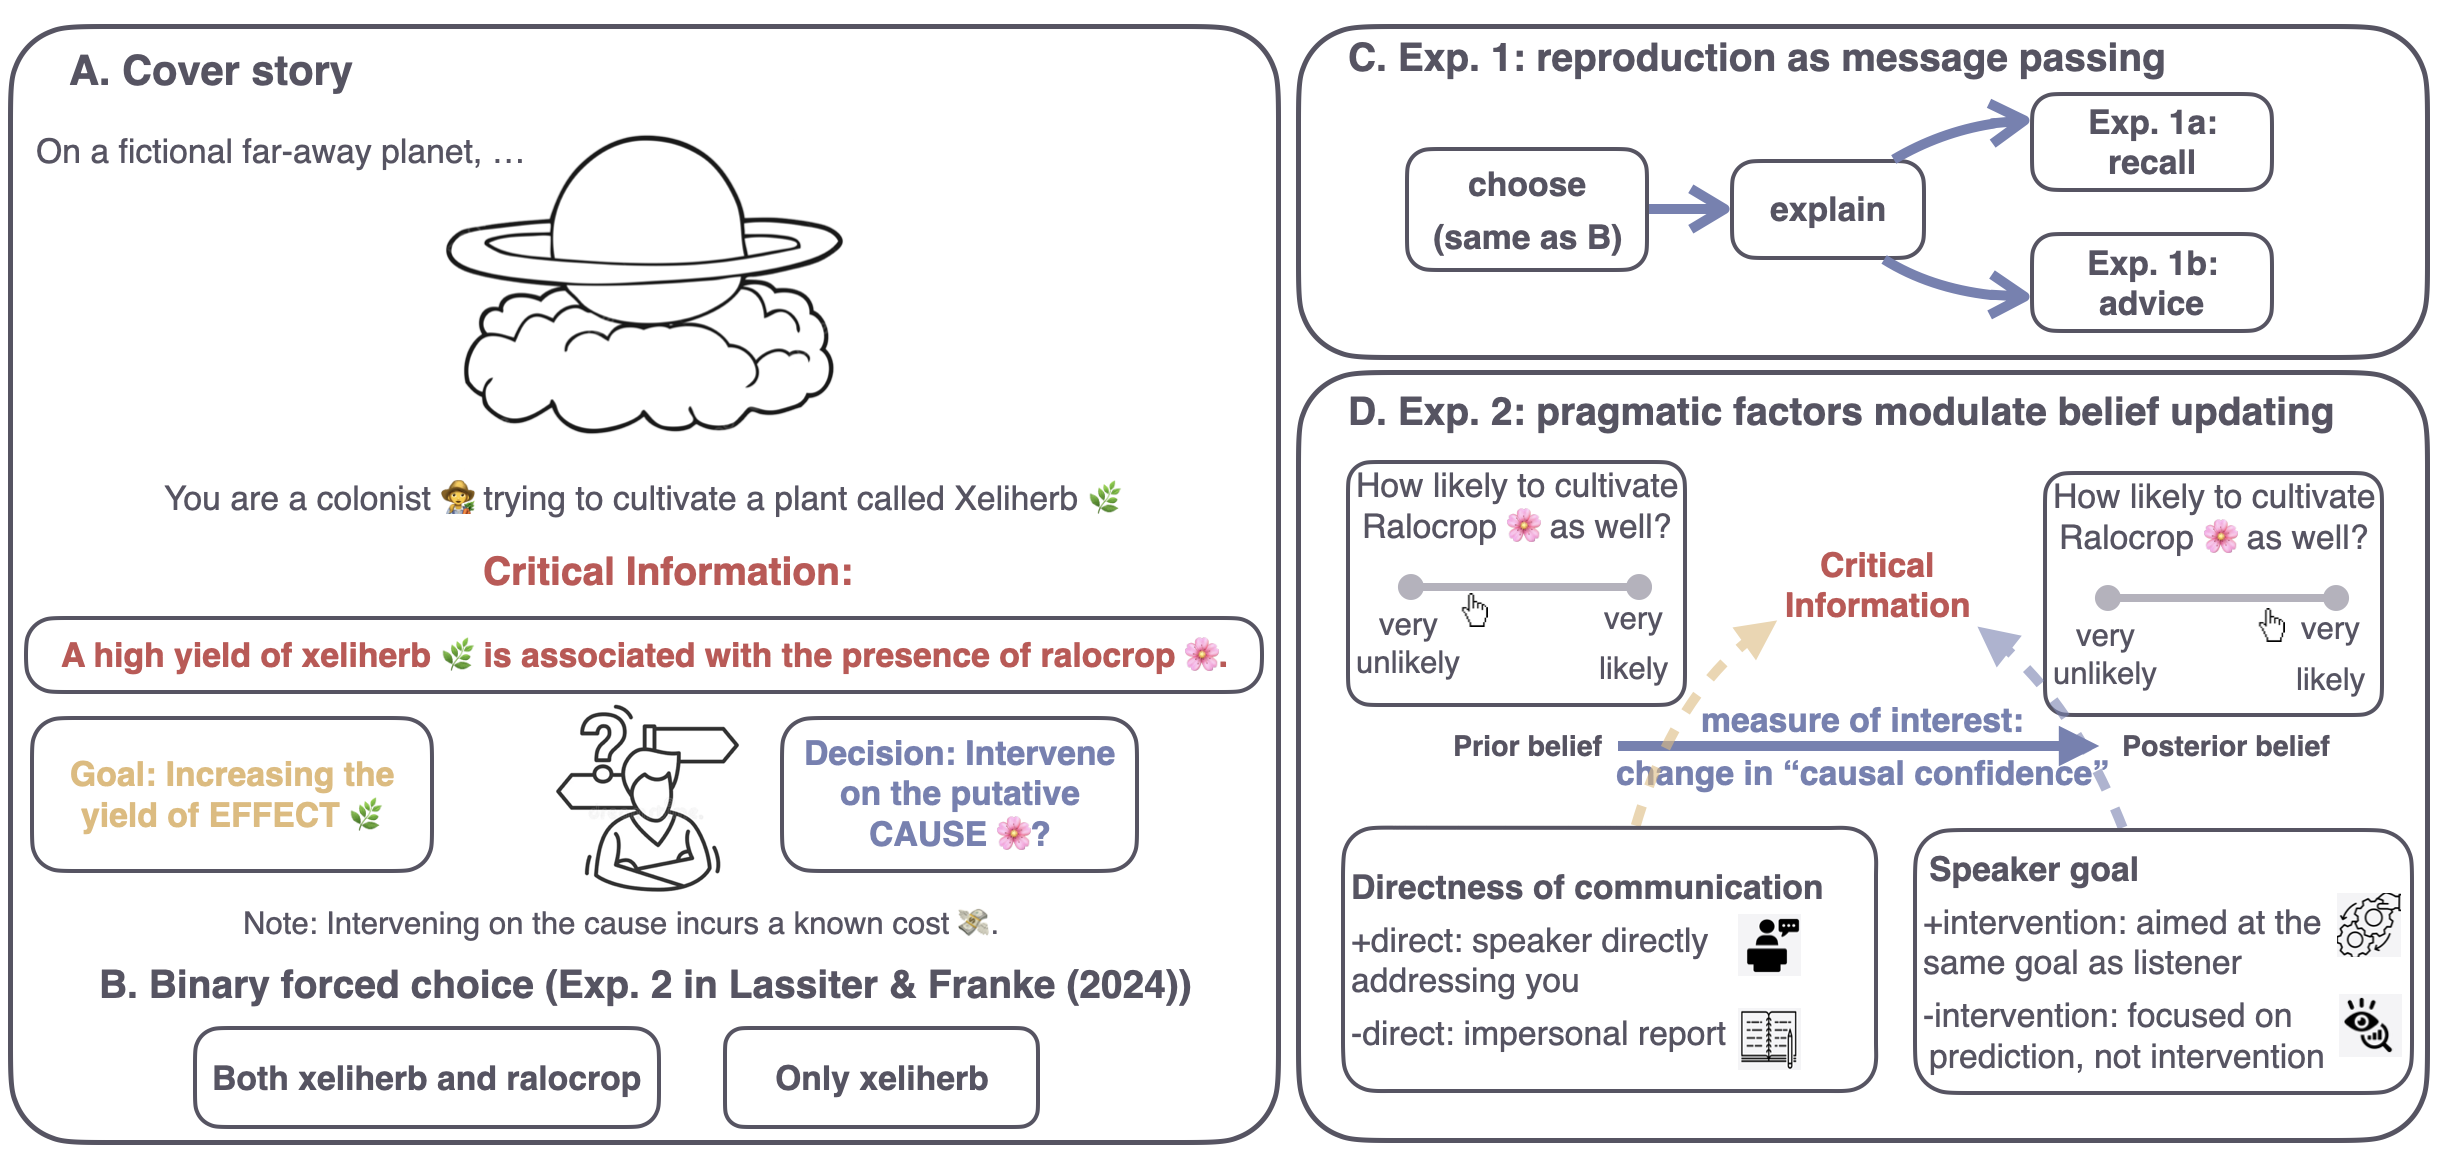
\includegraphics[width=0.875\linewidth]{figures-exp2/xeliherb_overview.png}
    \caption{Overview of the experimental paradigm across studies. 
\textbf{(A) Cover story and critical information:} Participants were placed in a fictional space-colonization scenario in which they aimed to increase the yield of a target plant (\textit{xeliherb}). They received correlational information stating that a high yield of \textit{xeliherb} is associated with the presence of another plant (\textit{ralocrop}). 
\textbf{(B) Binary forced-choice task:} Participants chose whether to cultivate both plants (interpreted as intervening on the putative cause) or only \textit{xeliherb}. 
\textbf{(C) Experiment~1: message passing via free production:} After making the same choice as in (B), participants either recalled the information (Exp.~1a) or reproduced it as advice to another agent (Exp.~1b), allowing assessment of how correlational statements are reported from memory or communicated message passing. 
\textbf{(D) Experiment~2: belief updating under manipulation of pragmatic factors:} Participants provided slider ratings for their willingness to cultivate \textit{ralocrop} before and after the critical statement, interpretable as \textit{causal belief change}. Pragmatic factors—directness of communication and speaker goal orientation—were manipulated to test how context modulates causal belief updating.}
    \label{fig:overview}
\end{figure*}

\section{Introduction}

Most ``Stats 101'' courses eagerly warn that \textit{correlation does not mean causation}. 
Yet outside the classroom, correlational claims are rarely encountered as abstract, decontextualized statements. 
Instead, they appear in headlines, summaries of scientific findings, expert advice, or reports embedded in broader narratives. 
In such settings, interpretation is shaped not only by statistical knowledge, but also by background beliefs, assumptions about speakers’ goals, and general world knowledge. 
In line with this, a growing body of evidence shows that people often interpret correlational statements in causal terms, even when no explicit causal language is used \citep{adams2017readers,huff2023lie,seifert2022causal}.

This pattern invites a more nuanced interpretation of the above warning itself. 
A correlational statement does not assert a causal relationship, but neither does it rule one out. 
Following \citet{reichenbach1991direction}, one may hold that the truth of a correlational statement presupposes some kind of causal direction, however indirect. 
So, if speaker and listener know that information about direct causation is relevant, inferring causation from correlational language may be legitimate.

In recent work, \citet{gershman_causal_2023} experimentally showed systematic preferences in assigning cause and effect based on correlational statements like ``$A$ is correlated with $B$.''
This can be interpreted as suggestive evidence for \textit{causal implicatures}, which people draw automatically from correlation language.
However, related work on implicit causality shows that linguistic structure can systematically influence causal attribution \citep{hartshorne_what_2014,bott_verbs_2014} without necessarily invoking pragmatic implicatures, and follow-up work by \citet{lassiter2024rationality} argues that \citeauthor{gershman_causal_2023}'s findings are better conceptualized as a \emph{PACE effect} (Preferences in Assignments of Cause and Effect) rather than a genuine pragmatic inference.

However, \citeauthor{lassiter2024rationality} also provide positive evidence in favor of a \textit{pragmatic inference view} of causal enrichment of correlational statements.
Their experiment introduced a fictional space-colonization scenario in which a Science Team provided information for participants who then had to make an important (binary) decision (see Figure~\ref{fig:overview}A--B).
The scenario involved a plant called \textit{xeliherb} which is important for the space colonists' survival. 
In the critical condition, the Science Team presents an association statement of the form (\ref{bsp:association}),  where \textit{ralocrop} is another plant.
%
\begin{exe}
    \ex \label{bsp:association} A high yield of \textit{xeliherb} is associated with the presence of \textit{ralocrop}.
\end{exe}
%
Based on the received information, participants then had to choose from two options, namely to cultivate \textit{both} plants, or to \textit{only} cultivate \textit{xerliherb}. 
The experiment manipulated (between-subjects) the kind of information given in the Science Team's report, ranging from explicitly denied causation, through correlational association (as in (\ref{bsp:association})), to explicit intervention-based causal descriptions. 
Since cultivation of \textit{ralocrop} may be costly, a choice to cultivate \textit{both} plants is rational only to the extent that the decision-maker beliefs in a causal effect on the yield of \textit{xeliherb}. 
Evidence for a certain degree of \textit{causal belief} after the association statements comes from the observation that the proportion of choices of option \textit{both} after receiving (\ref{bsp:association}) was higher than after hearing a statement that explicitly denied a causal relationship, and indistinguishable from a statement that used interventionist language to communicate a strong sense of causal relation. 

While this study provides some evidence for the pragmatic inference view, this paper builds on the \textit{xeliherb}-paradigm by addressing two potential shortcomings and addressing more nuanced predictions of the pragmatic account.
%
First, the previous work has not yet shown conclusively that the imputed causal belief from correlational language also strongly affected anything beside the concrete forced-choice decision. 
For that reason, Experiment 1 reported in this paper examines how causal interpretations of correlational statements influence other subsequent decision, such as to repeat what the Science Team actually reported, or to give advice to other future decision makers. 
%
Second, the between-subjects forced-choice design does not provide a strong signal of the belief change triggered by correlation statements.
%
Moreover, the pragmatic account predicts that the degree of causal belief should be influenced systematically by contextual factors, such as the speaker's goal and whether the message was directed at the listener or merely overheard.
Experiment 2 therefore directly measures belief updating within individuals and tests how pragmatic features of the communicative context modulate causal enrichment. 
Across these experiments, we find that correlational statements can strengthen causal beliefs in decision-relevant contexts, that these beliefs are reflected in participants’ memory reports and action-guiding communication, and that their impact depends systematically on pragmatic features of the communicative context. 
Crucially, we identify not only the conditions under which causal interpretations are strengthened, but also those under which they are attenuated—patterns that provide converging support for a pragmatic account of causal implicature grounded in reasoning about speakers’ communicative intentions and goals.


\begin{comment}
    

\section{Experiment 1}
\todo{Write about how Experiment 1 is arranged into sub experiments}

\subsection{Methods}
\subsubsection{Participants}
We recruited 200 participants via Prolific (English Native, at least 10 previous studies, at least 90\% approval rate and exclusions from previous pilot studies). For technical reasons that some data are not properly recorded upon submission, N=198 data sets were received for Exp. 1a, and N=203 for Exp. 1b. Participants took an average of 2.69 minutes for both Exp. 1a and Exp. 1b. They were paid 0.40 British Pounds. This and all subsequent experiments offered above-average compensation according to the platform.

\subsubsection{Design}

The experiment comprises four experimental conditions that differ in the report provided by the science team — specifically, in the sentence highlighted in bold in Figure~\ref{fig:exp1_item}. The conditions and their corresponding statements were as follows:

\begin{itemize}
    \item \textbf{Association}: ``A high yield of \textit{xeliherb} is associated with the presence of another plant called \textit{ralocrop}.''
    \item \textbf{Intervention}: ``A high yield of \textit{xeliherb} was obtained whenever another plant called \textit{ralocrop} was cultivated as well.''
    \item \textbf{Common Cause}: ``A high yield of \textit{xeliherb} is associated with the presence of another plant called \textit{ralocrop}. But they also found that \textit{ralocrop} only grows on particularly fertile grounds.''
    \item \textbf{Denied Causation}: ``A high yield of \textit{xeliherb} is associated with the presence of another plant called \textit{ralocrop}. But there is no evidence that the cultivation of \textit{ralocrop} causes a better yield of \textit{xeliherb}.''
\end{itemize}

The experiments differed only in whether the context description included (\textbf{Exp. 1b}) or excluded (\textbf{Exp. 1a}) additional information regarding the potential cost of cultivating the second plant. This is the second factor 

The scenario leaves underdetermined how large a potential gain from cultivating both plants is. Likewise, while Exp. 1b mentions a potential cost of cultivating both plants, the precise cost is also implicit. Nevertheless, it is reasonable to assume that, all else equal, the more likely a participant considers the relevant causal relation, the more likely they would select the “both” option. 

The condition of main interest is association. The other conditions function as reference categories. We expect different degrees of belief in the relevant causal relation (ralocrop causes a high yield of xeliherb) in different conditions. Concretely, we expect higher choice rates of the “both” option in the association condition than in the deniedCausation condition. The latter condition is intended to provide a lower bound on the strength of causal implicature. An upper bound on causal implicature strength is provided by the intervention condition, which is predicted to have the highest rates of the “both” choice, as it explicitly mentions effects observed after intervention. The commonCause condition makes only a very mild, suggestive gesture to a potential common cause of a high yield (fertile ground), and may thus be expected to lie in between the deniedCausation and the association condition. Since Exp. 1b additionally makes more salient a potential cost, we expect that choice rates for the ``both” option are generally lower.

\subsubsection{Materials}

The materials 
%\footnote{The experiment code, data an material are available online \todo{add link}. A live version of the experiment can be tested here. \todo{add link}} 
consist of linguistic contexts structured as follows: a running cover story, a critical sentence modulated by experimental condition, and a follow-up question, as illustrated in Fig.~\ref{fig:exp1_item}. The cover story introduces a fictional Sci-Fi scenario in which participants imagine themselves as colonists on an alien planet. Their goal is to cultivate an essential plant, \textit{xeliherb}, whose yield may be affected by the presence of another plant, \textit{ralocrop}. This setup is intended to minimize the influence of participants’ prior causal knowledge while allowing for tight experimental control over the formation of perceived cause-effect relationships. The critical sentence, framed as a report from a science team, serves as the basis for introducing a correlational statement. The question that follows is a simple binary choice designed to elicit participants’ decisions.

\begin{figure}[htbp]
    \centering
    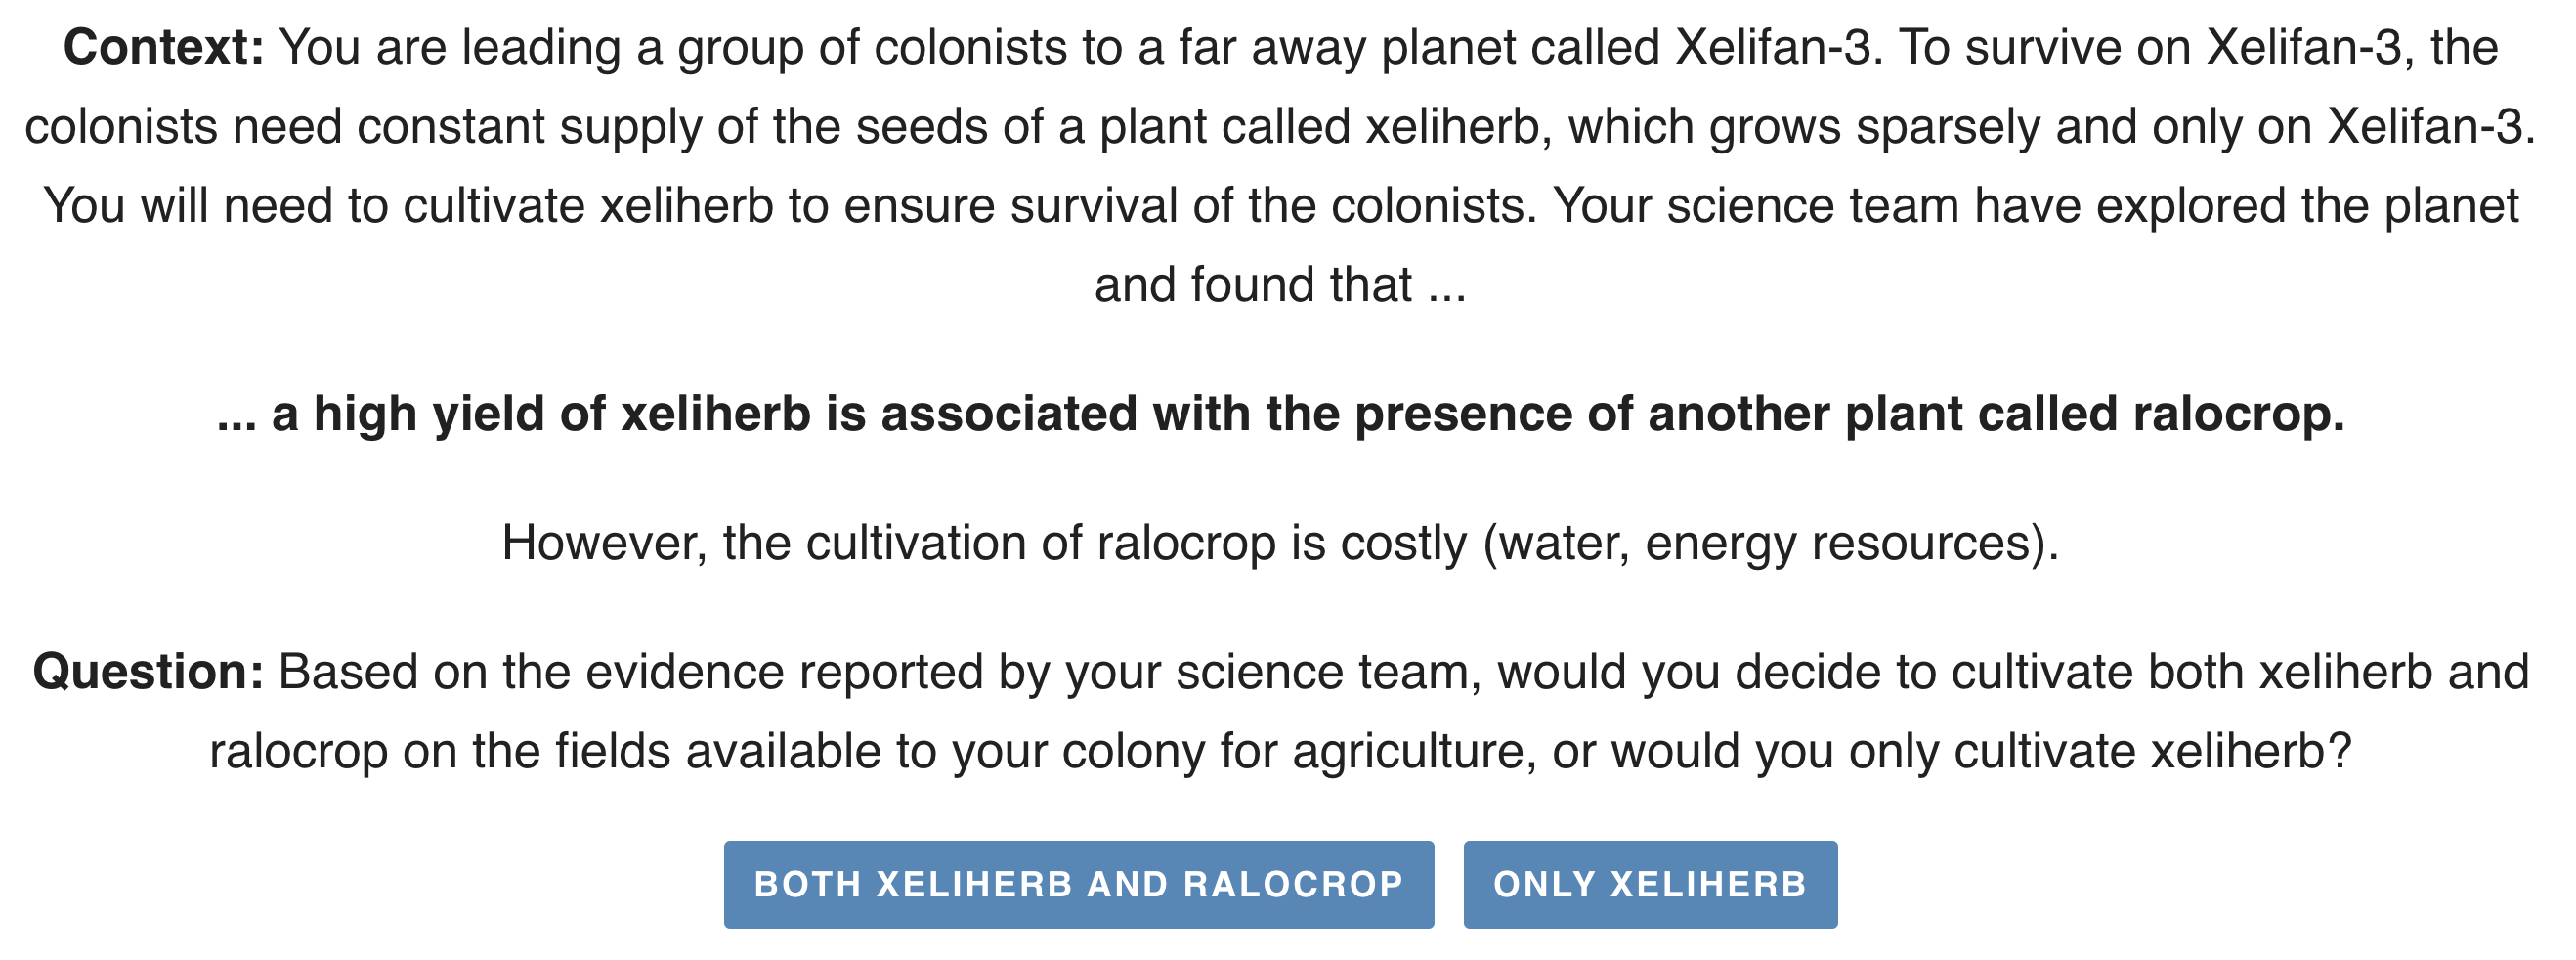
\includegraphics[width=0.9\linewidth]{figures-exp1/screenshot-trial-pilot-1b.png}
    \caption{A screenshot from main trial of Exp. 1b. For Exp. 1a the sentence regarding the cost of cultivating an additional plant ``However, the cultivation of ralocrop is costly." was omitted.}
    \label{fig:exp1_item}
\end{figure}


\subsubsection{Procedure}

The experiments employed a binary forced-choice task with a one-shot, between-subjects factorial design. Each participant was randomly assigned to one condition and completed a single trial. Responses were coded as 1 for choosing \emph{both} and 0 for choosing \emph{only}. After completing the task, participants provided demographic information and optional comments; these data were not included in the analyses.


\begin{figure*}[h!]
\centering


\begin{subfigure}[t]{0.48\textwidth}
    \centering
    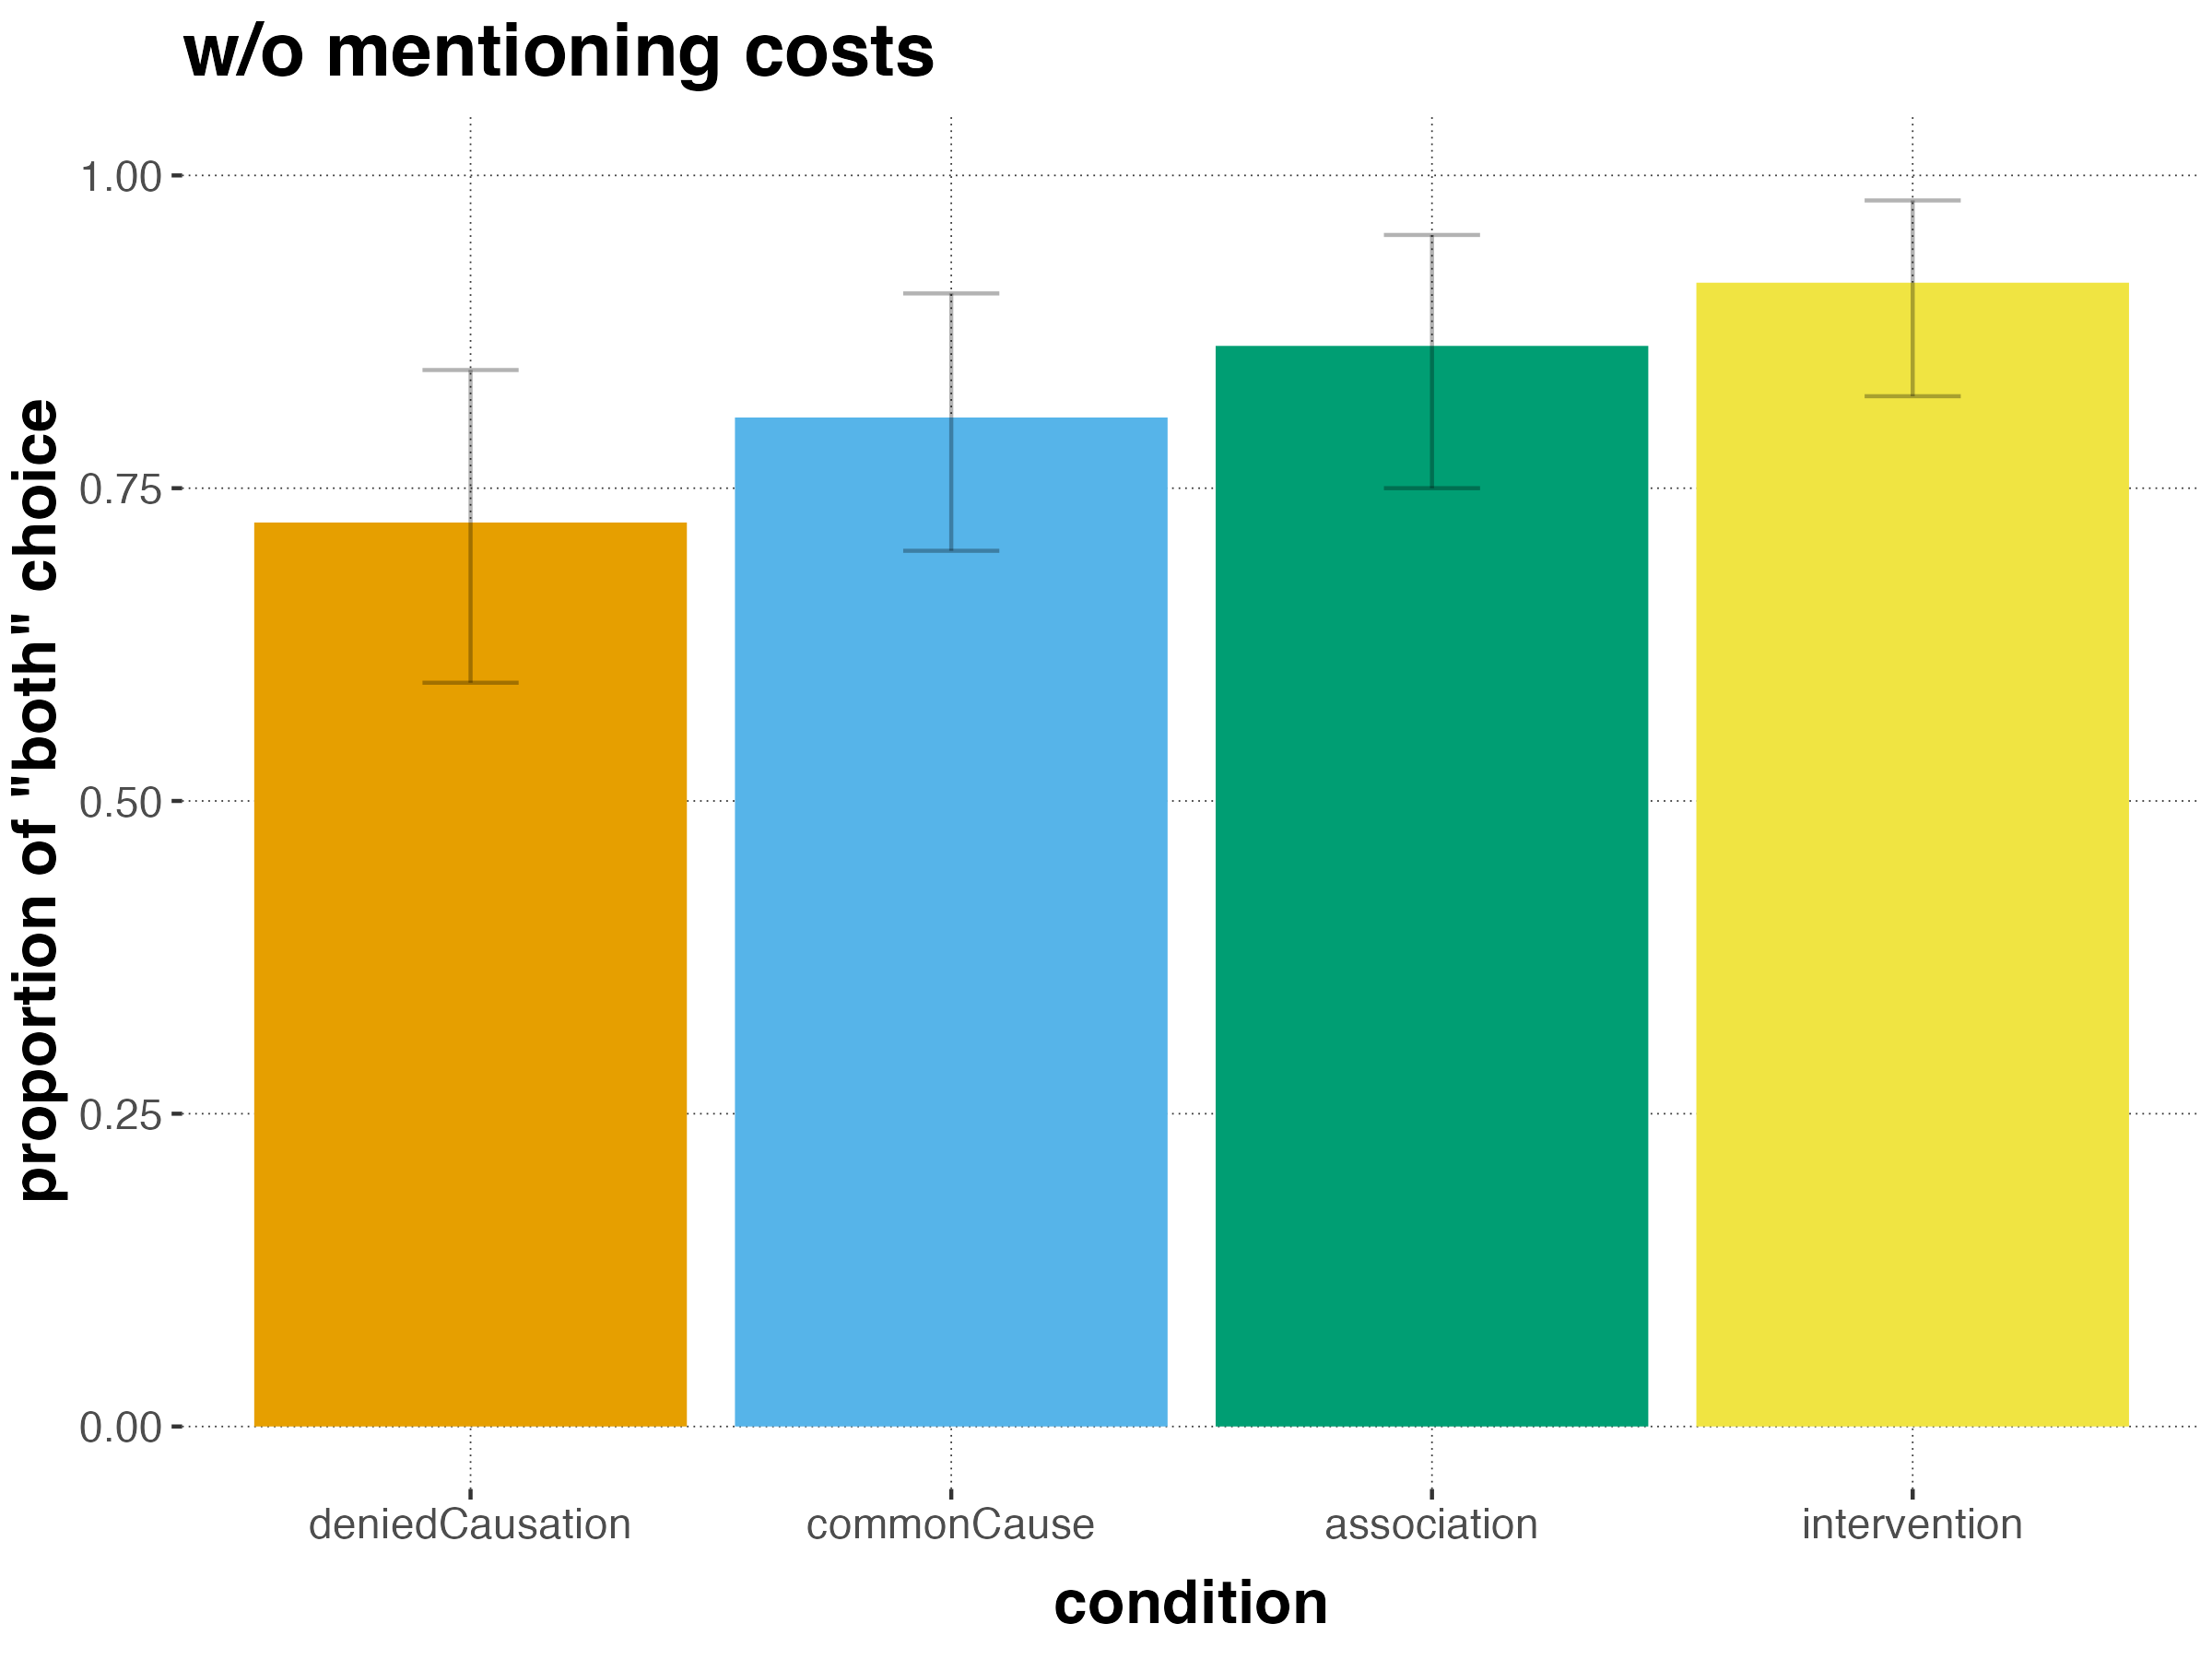
\includegraphics[width=\linewidth]{figures-exp1/result-exp1a.png}
    \caption{Experiment~1a}
    \label{fig:exp1a}
\end{subfigure}
\hfill
\begin{subfigure}[t]{0.48\textwidth}
    \centering
    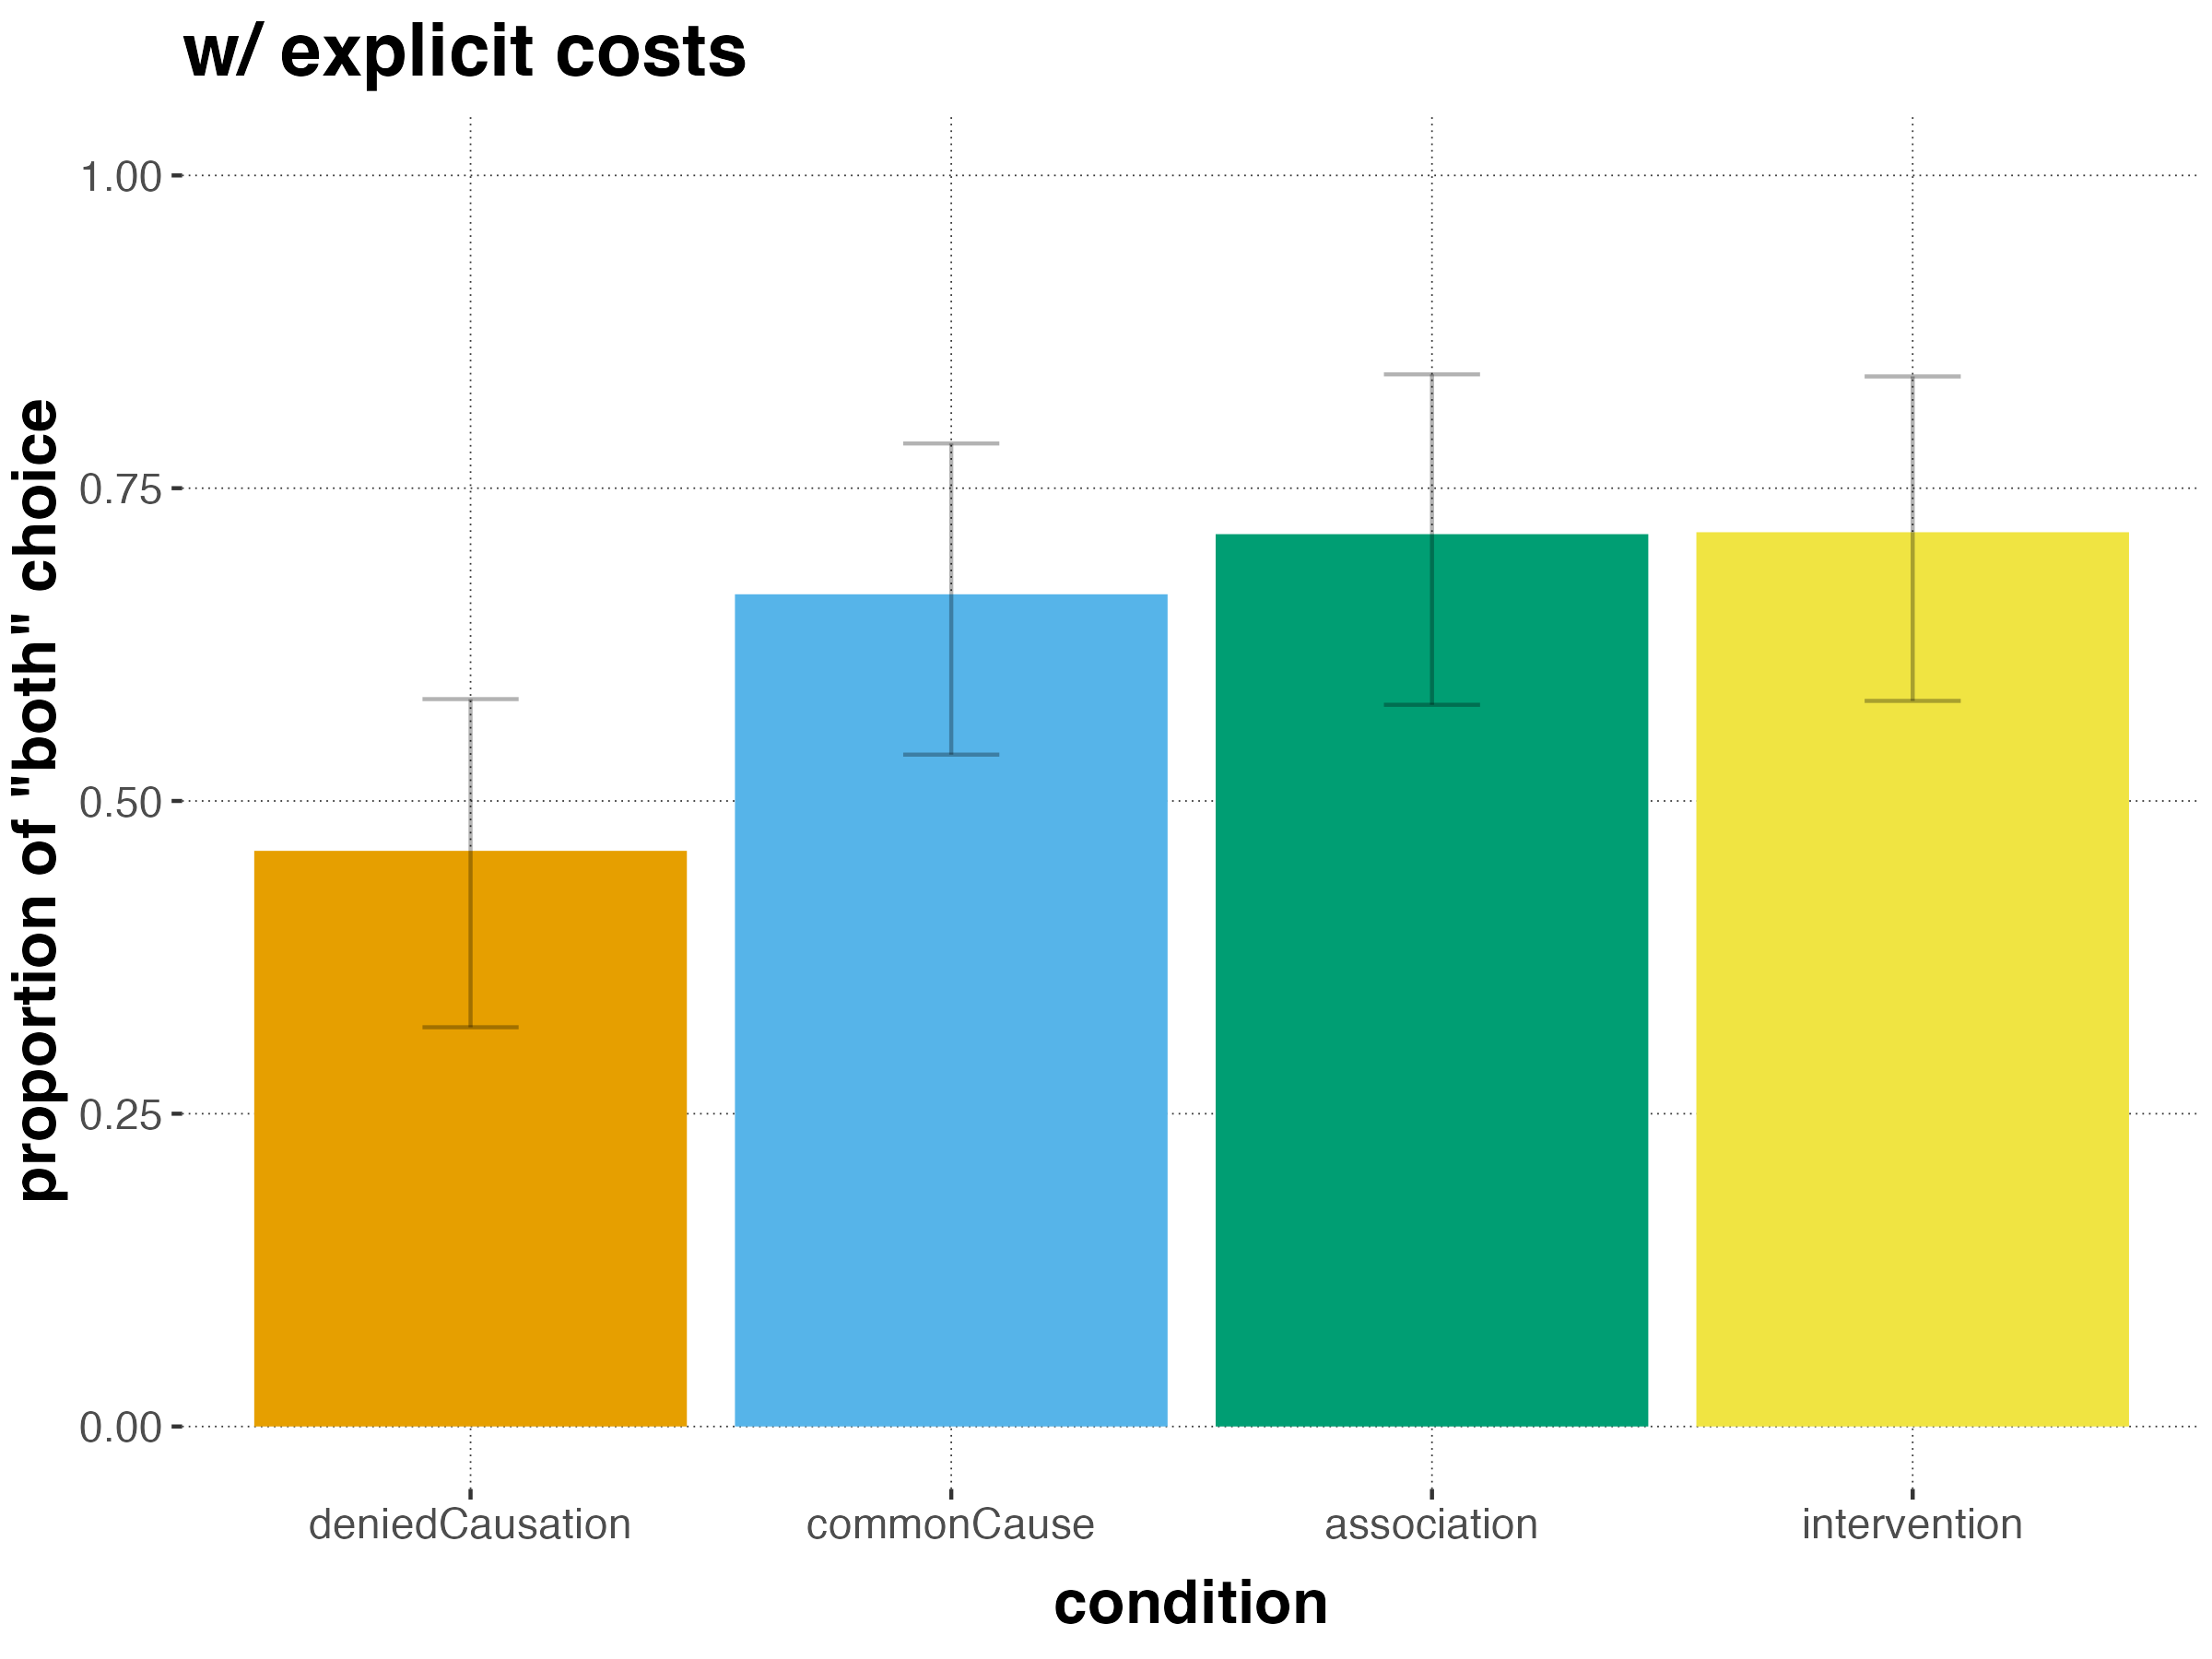
\includegraphics[width=\linewidth]{figures-exp1/result-exp1b.png}
    \caption{Experiment~1b}
    \label{fig:exp1b}
\end{subfigure}

\vspace{1ex}
\caption{Mean proportion of ``both'' choices across conditions in Experiments~1a and~1b. Error bars indicate bootstrapped confidence intervals for the mean.}
\label{fig:results_exp1}
\end{figure*}

\subsection{Results}
\todo{Expand this part?}

Fig. \ref{fig:results_exp1} shows the proportions of \emph{both} choices. We find that participants respond with a choice option indicating an increased degree of belief in a causal relation more often for the association condition than for the deniedCausation condition. However, in a Bayesian logistic regression model this contrast is only credible for Exp. 1b, i.e., when the cost of additionally cultivating another plant are salient. The posterior probability for contrast deniedCausation < association was 0.96 with 95\% credible interval of difference [-0.11; 2.08] for Exp. 1a, and 0.99 ([0.26; 1.98]) for Exp.1b. Moreover, the contrast association < intervention is not credible in either experiment (0.76, [-0.82; 1.95] for Exp. 1a, and 0.52, [ -0.92; 0.92] for Exp. 1b). The full results of the regression analyses are in Table \ref{tab:exp1_results}.

\begin{table}[ht]
\caption{Pairwise Comparisons of Causal Belief Ratings in Experiments 2a and 2b}
\label{tab:exp1_results}
\centering
\begin{tabular}{lcc}
\toprule
\textbf{Comparison} & \textbf{Exp. 1a} & \textbf{Exp. 1b} \\
\midrule
\texttt{denC < comC}     & 0.87, [--0.36 ; 1.46]     & 0.98$^{**}$, [0.13 ; 1.68] \\
\texttt{comC < ass}      & 0.78, [--0.67 ; 1.58]     & 0.68, [--0.64 ; 1.08] \\
\texttt{ass < inter}     & 0.77, [--0.89 ; 1.85]     & 0.52, [--0.90 ; 0.93] \\
\texttt{denC < ass}      & 0.96$^{*}$, [--0.11 ; 2.08] & 0.99$^{**}$, [0.22 ; 1.94] \\
\texttt{denC < inter}    & 1.00$^{**}$, [0.33 ; 2.87]  & 0.99$^{**}$, [0.29 ; 1.93] \\
\bottomrule
\end{tabular}

\vspace{1ex}
\raggedright
\textit{Note.} Values indicate posterior probability of difference in predicted means, with 95\% credible intervals in brackets.\\
$^{*} p > .95$, $^{**} p > .99$
\end{table}

\subsection{Discussion}
\todo{Revise this part under the big picture of the story}

Exp.1 suggests that statements of association can influence practical decision making to a similar extent as descriptions of intervention effects. It could be objected that the data are in principle compatible with the idea that mere mentioning of “ralocrop” alone increases belief in a potential causal connection, and that a statement of association, while not actually increasing beliefs in a causal connection, merely only decreases beliefs to a certain extent. Nevertheless, the studies show a behavioral effect that hints at different degrees of causal beliefs triggered by different linguistic expressions, some with a clearly non-causal literal meaning.
\end{comment}
\section{Experiment 1}

%Experiment~1 is designed to examine how participants’ \emph{own interpretations} of correlational statements extend beyond their immediate decision responses, both in a recall task and in a downstream advice task (see Figure~\ref{fig:overview}C). 
In the \textit{xeliherb}-paradigm, choosing to cultivate \emph{both} plants is consistent with a causal interpretation of the correlational information (see Figure~\ref{fig:overview}B). 
However, such choice behavior provides only indirect evidence and does not reveal how participants construe the relationship expressed by the correlational statement once the immediate decision is made. 
In particular, it remains unclear whether acting on the putative cause reflects a transient response strategy tied to the task, or a more stable interpretation that participants are willing to reconstruct and communicate to others.
To address this gap, Experiment~1 elicits participants’ interpretations through free production after they underwent the same binary decision task as in prior work by \citet{lassiter2024rationality}.
Experiment~1a focused on recall of the previously encountered information, targeting how participants reconstruct the message they understood themselves to have received. 
Experiment~1b required participants to reproduce the information as advice, thereby engaging communicative use under action-oriented goals. By comparing production patterns across these tasks, Experiment~1 examines whether participants who choose to intervene are also more likely to recall correlational statements using explicit causal language. % explicitly causal terms when articulating their own interpretation.

\vspace{-.1in}

\subsubsection{Participants}

We recruited a total of 99 participants via Prolific. All participants were native English speakers, had completed at least 10 previous studies, and had an approval rate of at least 90\%; participants who had taken part in earlier pilot studies were excluded. Of these, $N = 49$ participated in Experiment~1a and $N = 50$ participated in Experiment~1b. Participants completed a single-trial experiment lasting approximately 5 minutes and were compensated \pounds0.90. This and all subsequent experiments offered above-average compensation according to the platform.

\subsubsection{Procedure}
The procudeure followed the general paradigm illustrated in Figure~\ref{fig:overview}A-C.
Participants first read the background story, followed by the critical correlational information. They then completed a binary forced-choice decision task in which they chose whether to cultivate \emph{only} \textit{xeliherb} (the effect) or \emph{both} \textit{xeliherb} and \textit{ralocrop} (the effect and the putative cause). Participants were additionally asked to provide a brief justification for their choice.

Following the decision task, participants completed the free-production task. In Experiment~1a, participants were asked to recall and pass on the information they had just read. In Experiment~1b, participants were asked to reproduce the information in the form of advice intended for another agent facing a similar decision. In both sub-experiments, the produced message was framed as being passed on to a subsequent recipient within the same fictional scenario.

\subsubsection{Materials}

Participants were first presented with the original \textit{xeliherb}-paradism (Experiment~2 from \citet{lassiter2024rationality}: see Figure~\ref{fig:overview}A). 
They received a report from a science team in the form of the correlational statement in (\ref{bsp:association}).
They decided between the options \textit{only xeliherb} and \textit{both}, where the latter indicates a sufficiently high degree of belief in causality, as described above. 
After completing the decision task, participants were prompted to produce a free-text message based on the information they had received. The wording of the prompt differed only with respect to the communicative goal. In Experiment~1a (recall), participants were instructed: %\mf{insert full instructions / scenarios for recall and message passing} \hw{done!}
%
\begin{quote}
\small
\emph{Due to atmospheric conditions and technical problems you are about to lose contact to an outpost on the planet. You have only very little time to send a short message to the colonists in this outpost before all contact breaks off for potentially a long time. The colonists in the outpost know about xeliherb and its importance. They know the costs associated with cultivation of ralocrop. What they do not know is what your Science Team reported. You cannot forward the original report. Please type what you recall from the Science Team's report into the text box, so that the other colonists can make a decision like you did on their own!}
\end{quote}
%
In Experiment~1b (advice), participants were instructed:
%
\begin{quote}
\small
\emph{There is also an outpost of your colonists on Xelifan-3. Unfortunately, due to atmospheric conditions, you can only send one message to the people in this outpost before all contact breaks off for potentially a long time. Tell the people in the outpost all they need to know about xeliherb and ralocrop, what they are good for, and how they might be related, so that they can decide what to cultivate for themselves!}
\end{quote}
%
Importantly, the recall task was not framed as reproducing the exact wording of the original message, but as reporting on the key information that had been communicated.
Under this interpretation of the task, reproducing the correlational statement in causal terms provides evidence that participants understood or construed the original message causally, rather than merely misremembering its surface form.
We therefore expect that participants who adopt a causal interpretation of the correlational statement—as indexed by their decision to intervene—will more often reproduce the information in explicitly causal terms in the recall task, and will more often convey causality-implying information in the advice task.





% \begin{figure*}[t]
% \centering
% \begin{subfigure}[t]{0.49\textwidth}
%     \centering
%     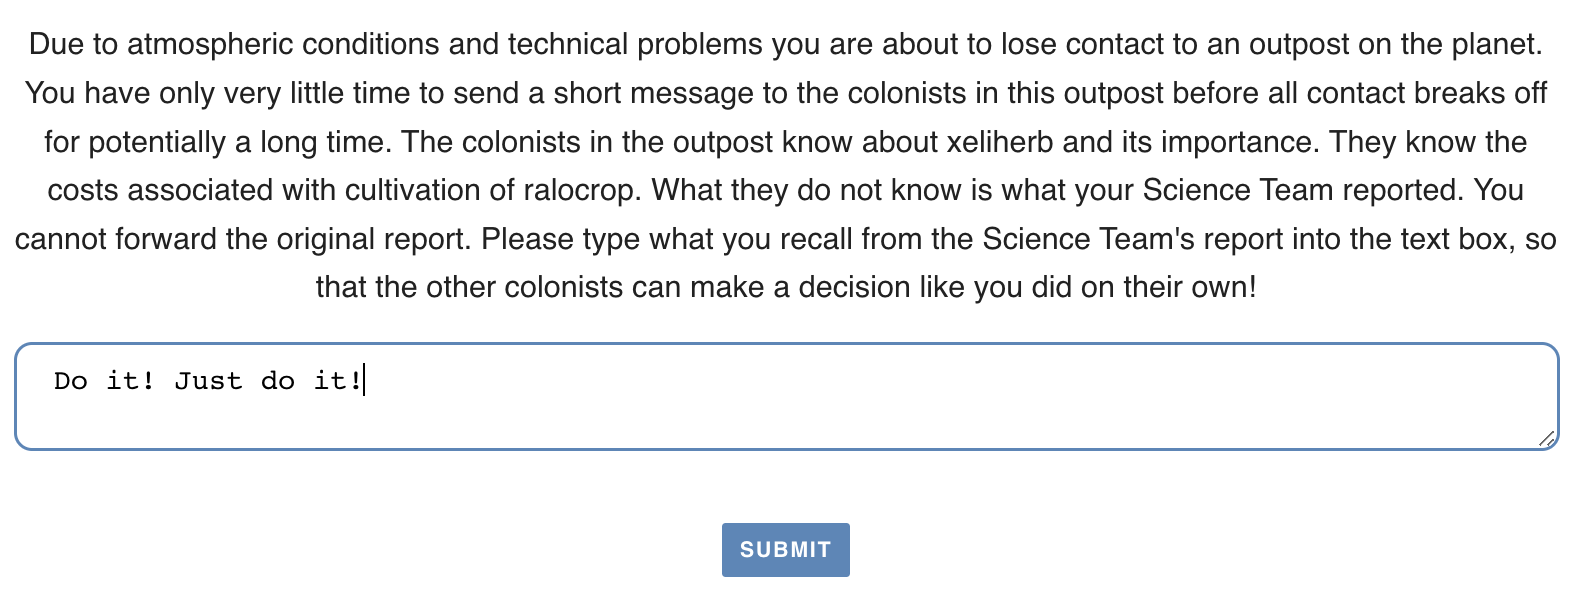
\includegraphics[width=\linewidth]{figures-exp2/screenshot-reprocution-trial-pilot-02a.png}
%     \caption{Experiment~1a: recall task}
%     \label{fig:exp1a}
% \end{subfigure}
% \hfill
% \begin{subfigure}[t]{0.49\textwidth}
%     \centering
%     \vspace{-8em}
%     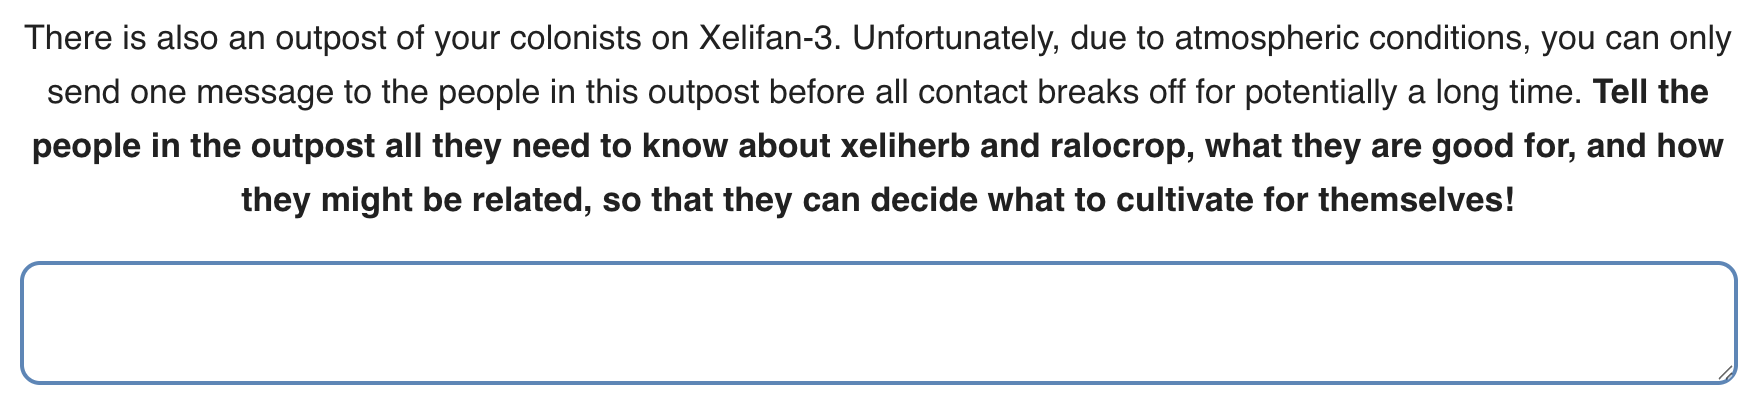
\includegraphics[width=\linewidth]{figures-exp2/screenshot-reporduction-04a.png}
%     \caption{Experiment~1b: advice task}
%     \label{fig:exp1b}
% \end{subfigure}
% \vspace{1ex}
% \caption{Screenshots illustrating the tasks used in Experiments~1a and~1b. Participants produced free-text messages that were subsequently passed on to another agent in the experimental scenario.}
% \label{fig:exp1_materials}
% \end{figure*}
% \begin{figure*}[t!]
% \centering
% \begin{subfigure}[t]{0.48\textwidth}
%     \centering
%     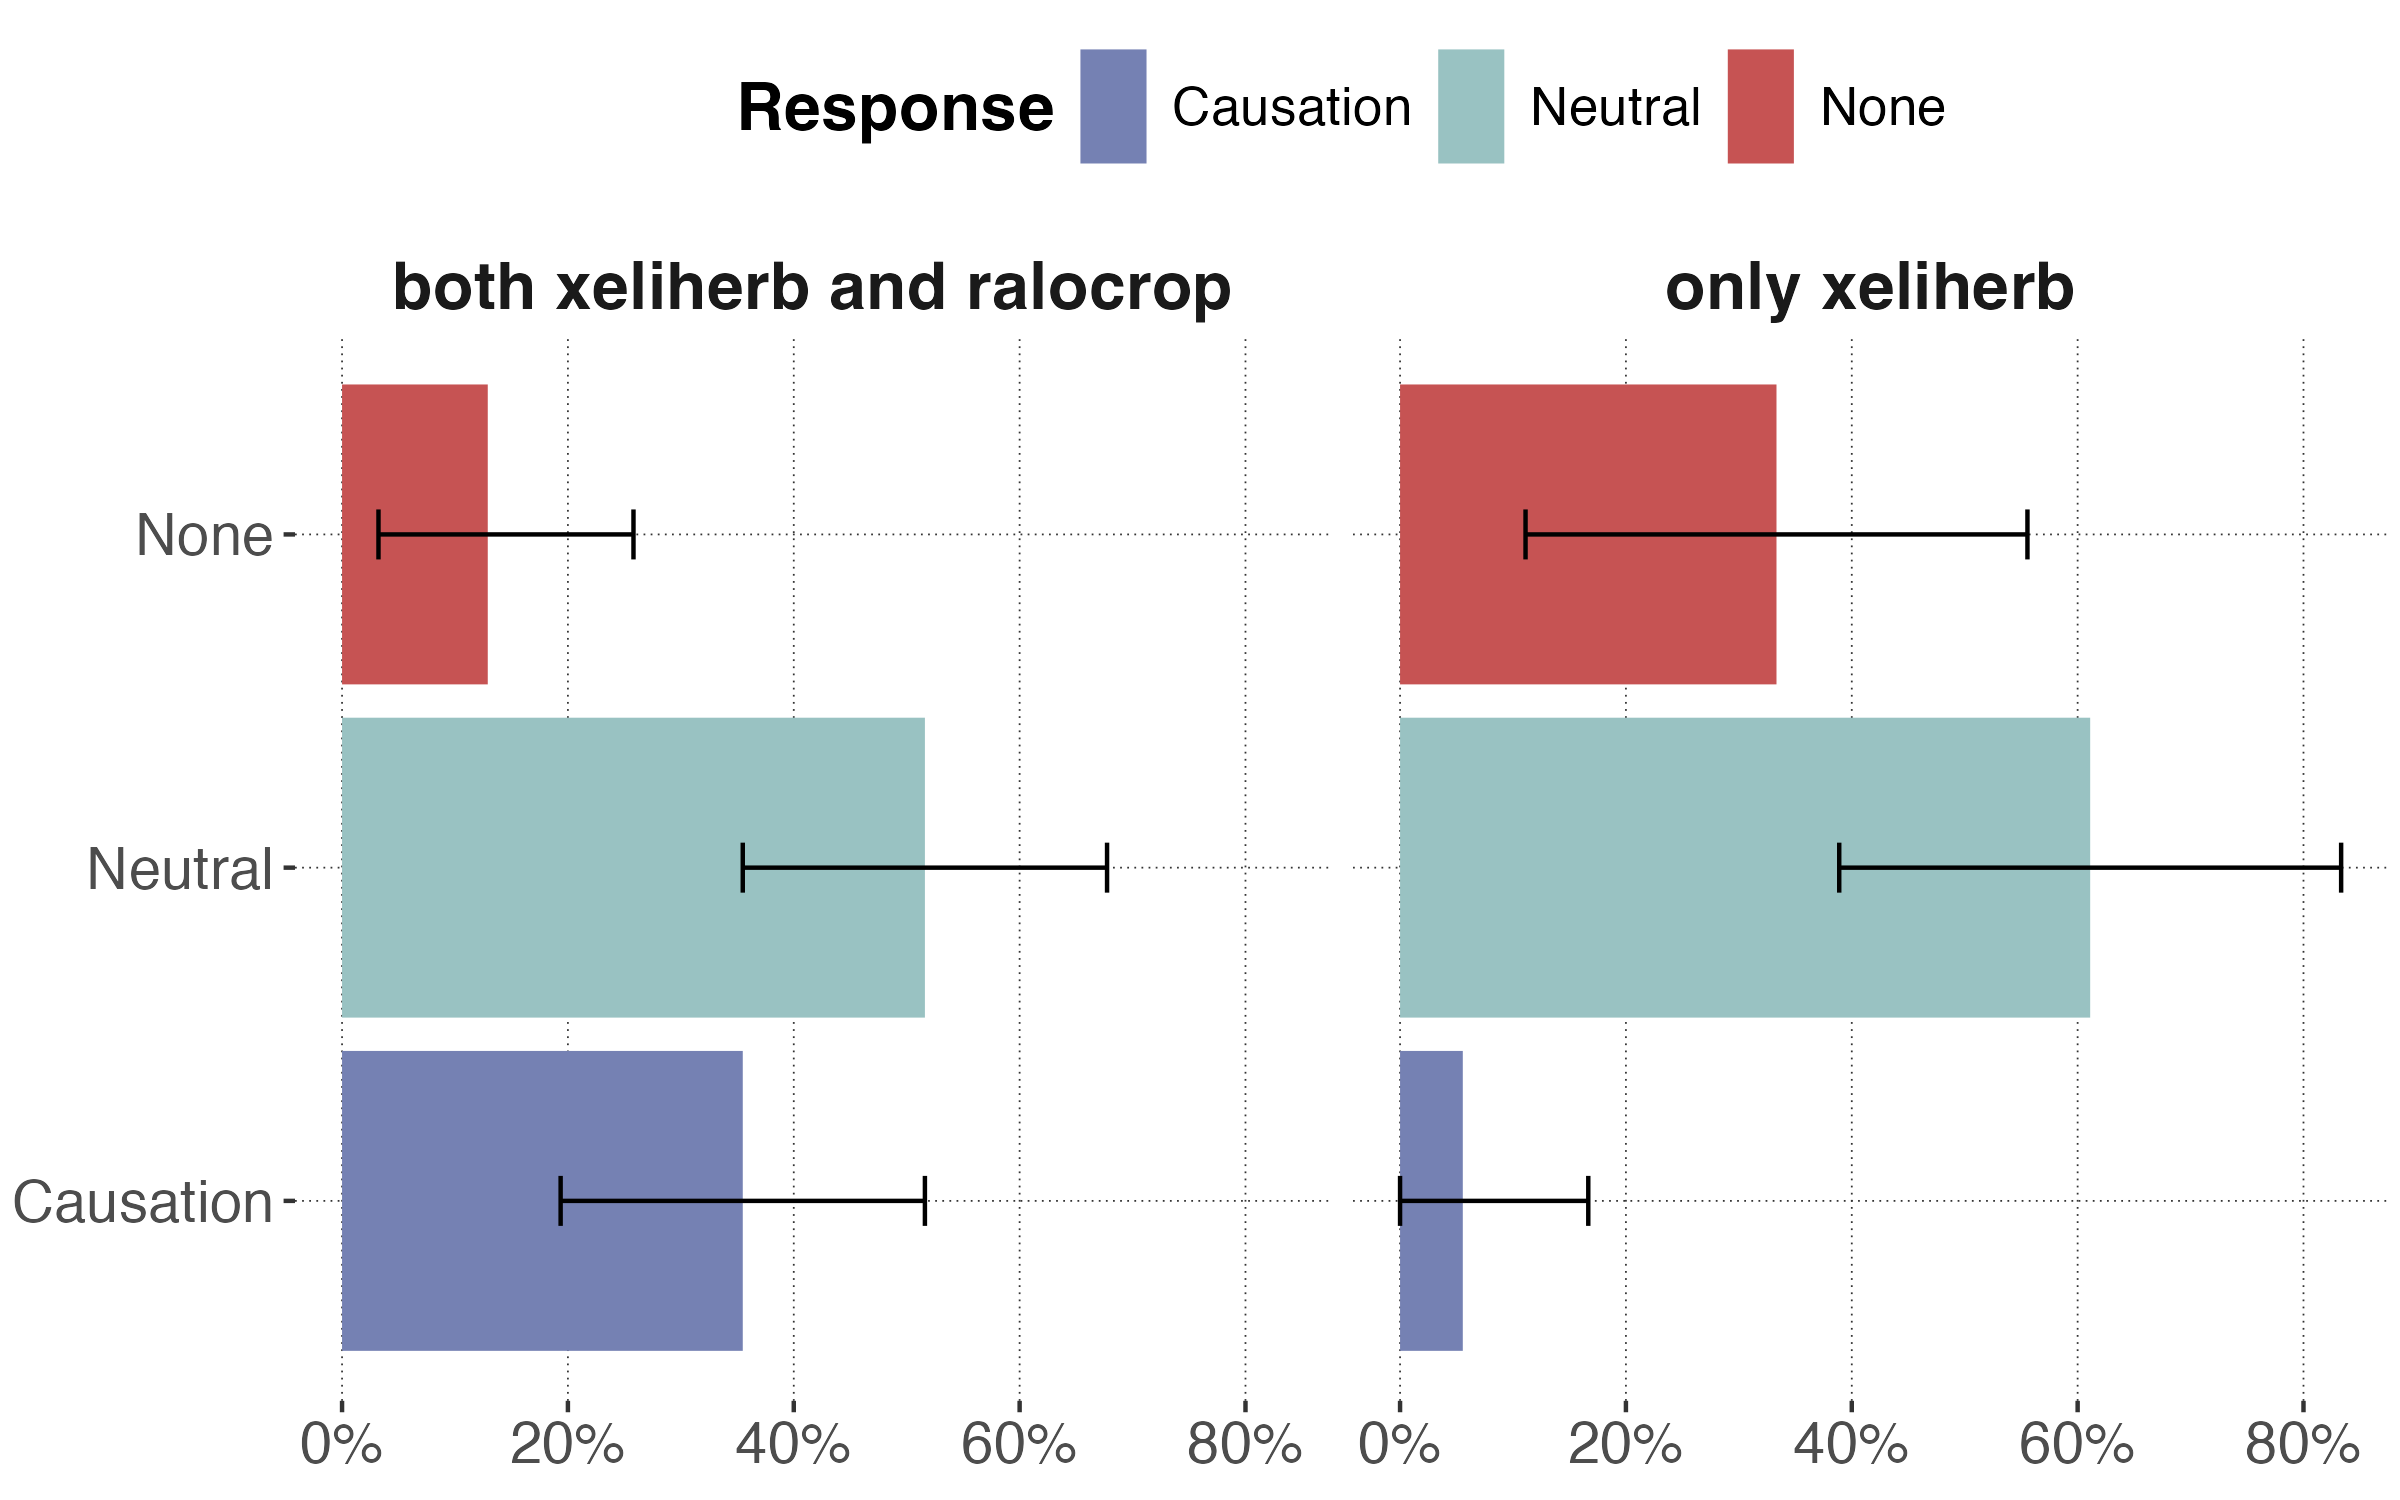
\includegraphics[width=\linewidth]{figures-exp2/results_exp2a.png}
%     \caption{Experiment~1a: choose-explain-recall}
%     \label{fig:results_exp1a}
% \end{subfigure}
% \hfill
% \begin{subfigure}[t]{0.48\textwidth}
%     \centering
%     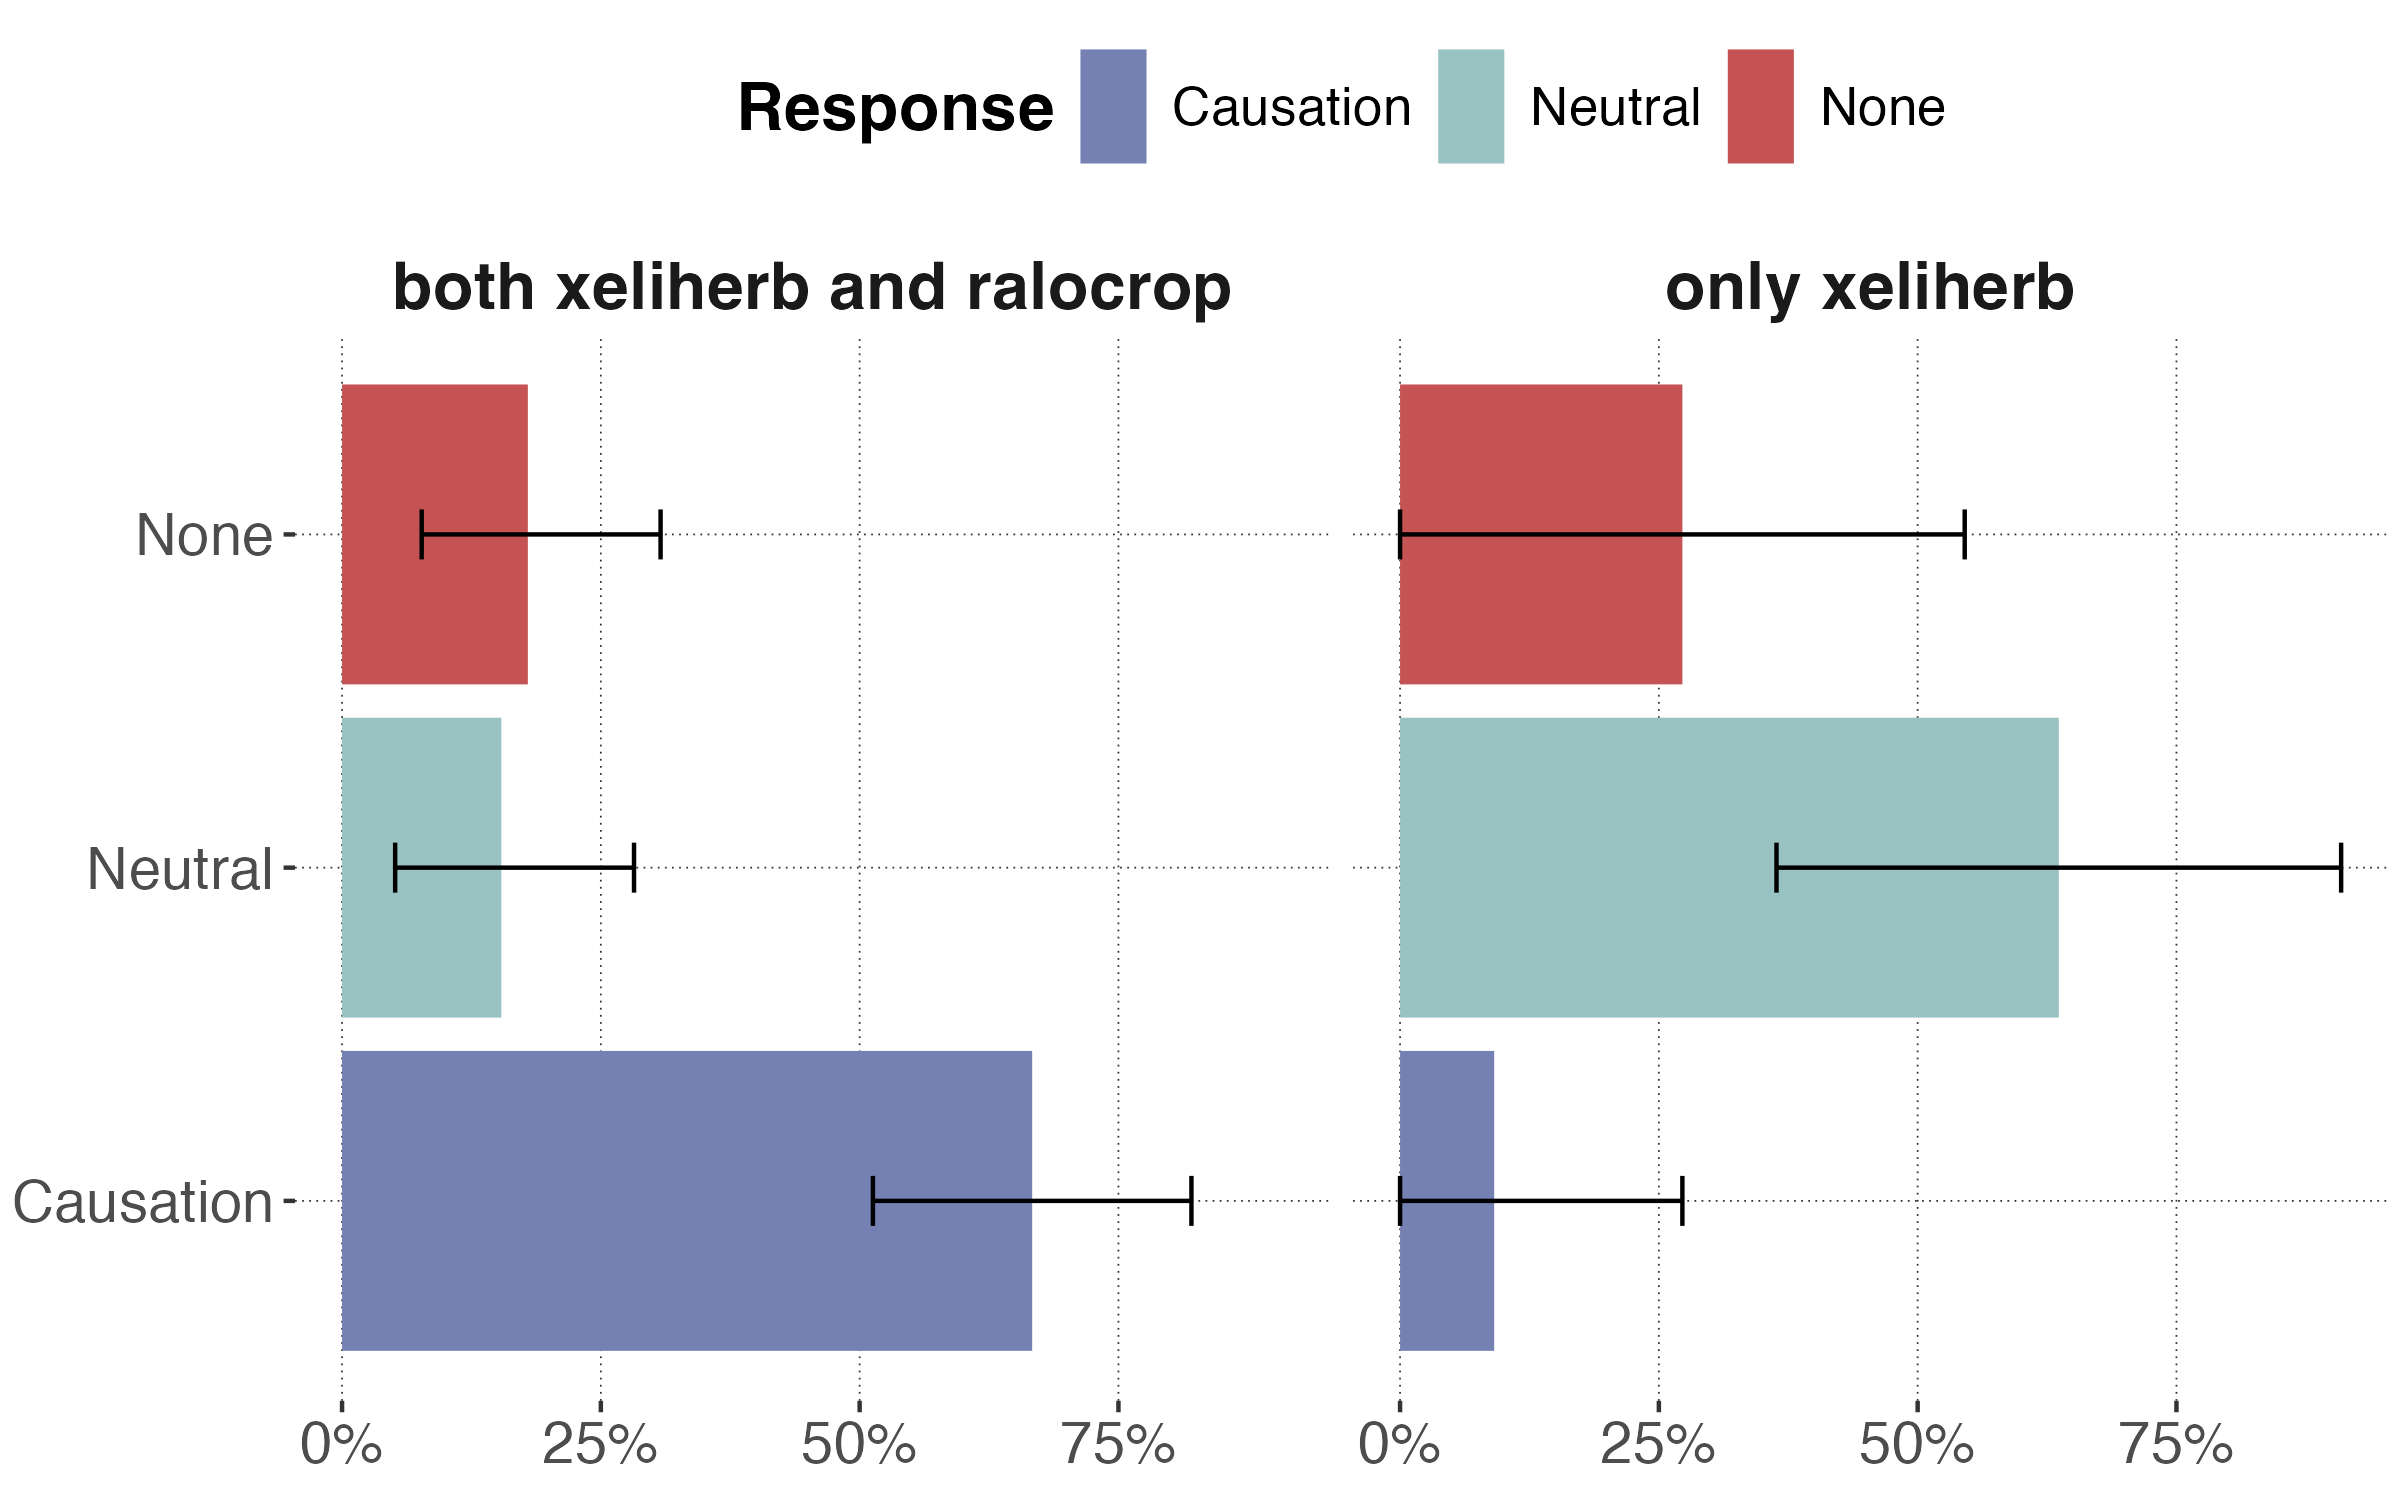
\includegraphics[width=\linewidth]{figures-exp2/results_exp2b.png}
%     \caption{Experiment~1b: choose-explain-advice}
%     \label{fig:results_exp1b}
% \end{subfigure}

% \vspace{1ex}
% \caption{Proportions of annotated response categories in Experiments~1a and~1b, split by participants’ initial choice in the decision-making trial (\emph{both} \textit{xeliherb} and \textit{ralocrop} vs.\ \emph{only} \textit{xeliherb}). Bars denote bootstrapped 95\% confidence intervals.}
% \label{fig:results_exp1}
% \end{figure*}

\begin{figure}
    \centering
    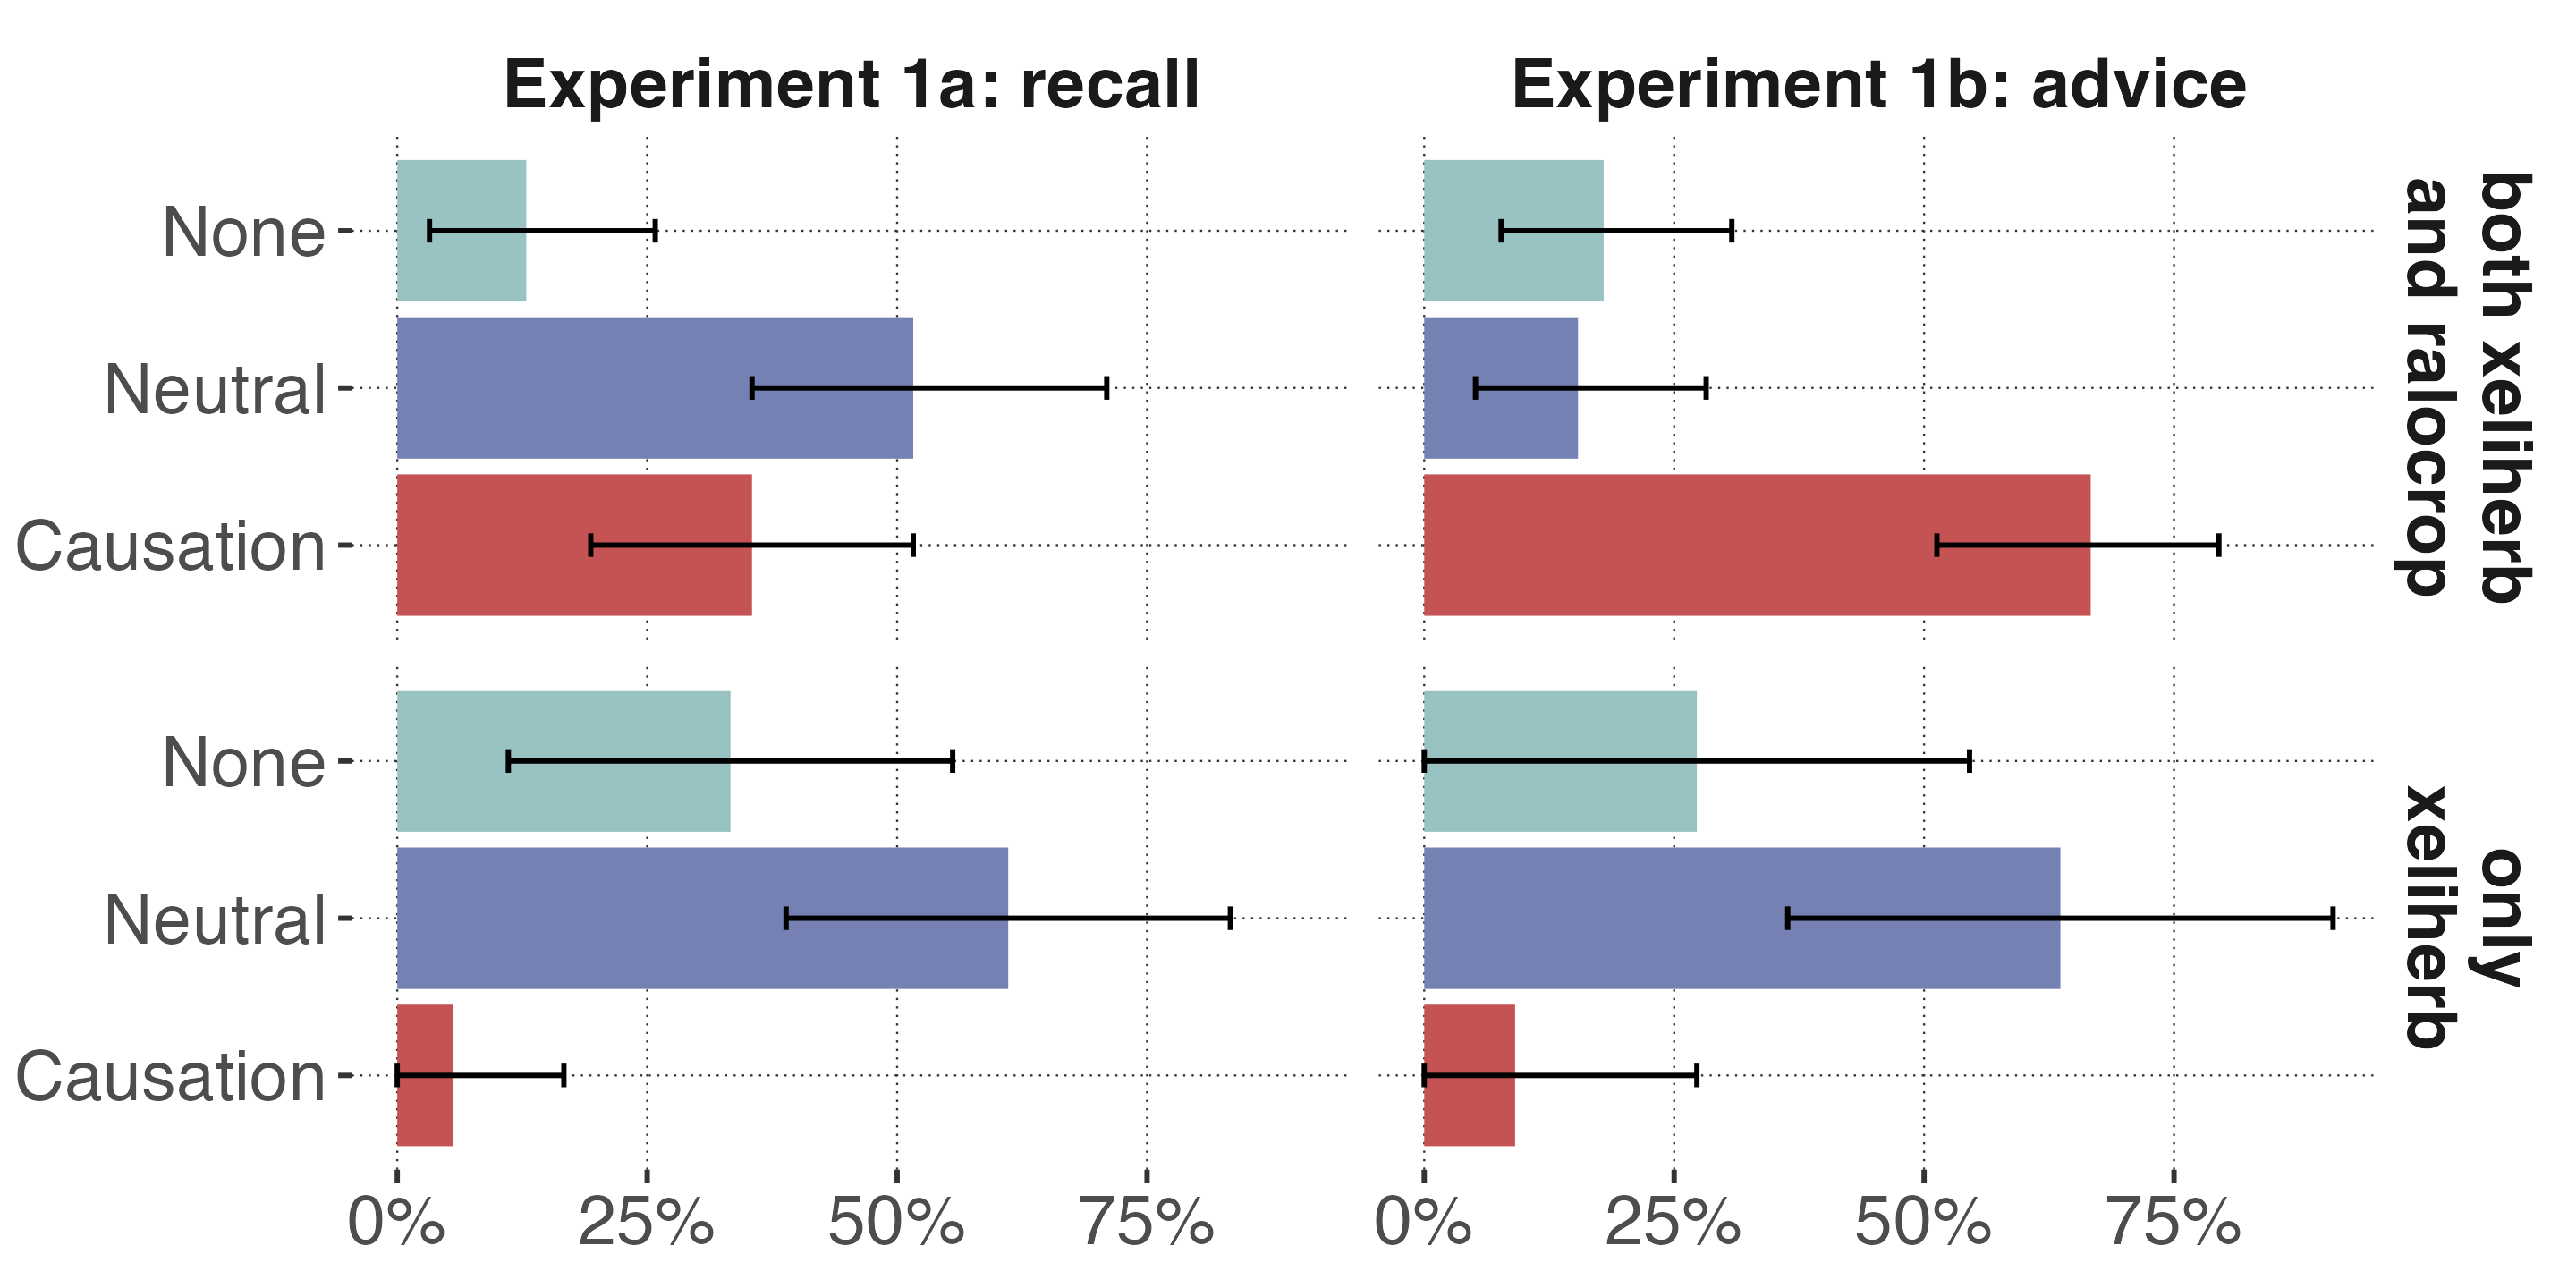
\includegraphics[width=\linewidth]{figures-exp2/results_exp2_combined.png}
    \caption{Proportions of annotated response categories in Experiments~1a,b, split by participants’ initial choice in the decision-making trial (\emph{both} \textit{xeliherb} \textit{and} \textit{ralocrop} vs.\ \emph{only} \textit{xeliherb}). Bars are bootstrapped 95\% confidence intervals.}
\label{fig:results_exp1}
\end{figure}


\subsubsection{Results}

Figure~\ref{fig:results_exp1} summarizes the results from the free-production recall task in Experiment~1a and the advice task in Experiment~1b. All free-production responses were manually annotated into three categories: \textit{causation}, \textit{neutral}, and \textit{none}, illustrated here with examples:

\begin{enumerate}
\item \textbf{None}: ``Ralocrop needs a lot of water, so I would just focus on xeliherb for now.''     
\item \textbf{Neutral}:`` If ralocrop grows, then xeliherb grows too.''
\item \textbf{Causation}: ``Xeliherb needs ralocrop in order to grow.''
\end{enumerate}

For hypothesis testing, responses coded as \textit{causation} were assigned a value of 1, and all other response categories were assigned a value of 0. We fit a generalized Bayesian regression model using \texttt{brms} \citep{brms} in \textsf{R} \citep{R-core}, including participants’ initial choice (\emph{both} \textit{xeliherb} \textit{and} \textit{ralocrop} vs.\ \emph{only} \textit{xeliherb}) as a predictor. Inference was based on posterior expected predictions.

In Experiment~1a, the majority of recall responses were classified as \textit{neutral} irrespective of participants’ initial choice. However, participants who initially chose \emph{both} \textit{xeliherb} \textit{and} \textit{ralocrop} produced a higher proportion of \textit{causation} responses than participants who chose \emph{only} \textit{xeliherb} ($\mu = 1.68$, CrI $[0.36, 3.08]$, posterior probability $= .98$).

In Experiment~1b, responses showed a clearer differentiation between choice groups. Participants who selected \emph{only} \textit{xeliherb} in the first decision-making task predominantly produced \textit{neutral} responses. By contrast, participants  who initially chose \emph{both} most frequently produced \textit{causation} responses, with a credibly higher rate than in the \emph{only} group ($\mu = 2.37$, CrI $[1.07, 3.79]$, posterior probability $= .99$).

\subsubsection{Discussion}

In both experiments, free-production responses varied systematically with participants’ initial choices, indicating how correlational information was recalled and communicated under different task demands.

In Experiment~1a, recall responses largely reproduced the correlational formulation, which is expected given that the original message was itself neutral. Importantly, however, participants who chose \emph{both} were more likely to produce causal paraphrases than those who chose \emph{only}. One interpretation is that the recall task was not treated as a verbatim memory test, but rather as a request to convey the intended message or meaning as understood in context. On this view, the use of causal language in recall responses reflects participants’ interpretations of the correlational statement, rather than a failure to remember its surface form. The observed difference between choice groups is therefore consistent with the possibility that participants who opted to intervene interpreted the original statement as conveying causal information.

This contrast was more pronounced in Experiment~1b, where participants were asked to reproduce the information as advice for another agent. In this communicative context, participants in the \emph{both} group most often produced explicitly causal messages, whereas participants in the \emph{only} group largely refrained from doing so. Because the advice task requires tailoring information to another agent’s presumed needs, these results suggest that causal interpretations were not only internally available but also selectively externalized when action relevance was salient.

%\DL{Please see note in Overleaf - I'm unsure if we are really warranted in interpreting the pattern of results in 1a as giving evidence about memory representations. But it definitely gives evidence about how the statement was interpreted, which is enough for our purposes.}

\section{Experiment 2}

Previous experiments established that correlational statements can support causal interpretations, as reflected in binary intervention choices and in how participants reproduce and communicate information. However, these measures provide only indirect access to causal belief and do not track how strongly such beliefs are updated within individuals. In Experiment~2, we therefore move beyond categorical choices and 
%examine causal interpretation in a setting where participants must decide for themselves whether and to what extent to intervene on a potential cause.
introduce a belief-update paradigm that directly measures changes in participants’ willingness to intervene relative to an individually measured baseline. 
This approach allows us to assess whether exposure to correlational information produces a graded shift in degrees of belief in causal power rather than merely influencing discrete responses. In addition, Experiment~2 systematically manipulates pragmatic features of the communicative context—specifically, directness of communication and speaker goal orientation—to test how reasoning about communicative intent modulates causal belief updating, as suggested by the patterns observed in Experiment~1.

Experiment~2 employed a between-participants factorial design with two manipulated factors: \textsc{directness of information} and \textsc{speaker goal orientation} (see Figure~\ref{fig:overview}D).
%
\textsc{Directness of information} determined whether the correlational information was presented as communicative input explicitly addressed to the participant (the \emph{direct} condition) or encountered as impersonal evidence not tailored to a specific listener (the \emph{indirect} condition). This manipulation varied the extent to which participants could treat the information as the result of audience design and deliberate communicative choice, as opposed to merely informational content.
%
\textsc{Speaker goal orientation} manipulated the functional role that the correlational information played in the speaker’s task. In the \emph{intervention-oriented} condition, the speaker belonged to a cultivation team whose goal was to improve the yield of \textit{xeliherb}, a context in which acting on potential causes is directly relevant. In the \emph{diagnostic-oriented} condition, the speaker belonged to a localization team whose goal was to identify where \textit{xeliherb} naturally grows, a context in which correlational information is relevant in a purely diagnostic role.

\subsubsection{Participants}

We recruited a total of 404 participants via Prolific using the same eligibility criteria as in the previous experiment. Each participant completed a one-shot trial for a single instance of randomly assigned between-subject conditions. All participants were native English speakers.

\subsubsection{Materials}

The materials %\footnote{A live version of the experiment is available at \url{https://heningwang.github.io/Xeliherb/experiments/3a/}.} 
were framed in the same space-colonization scenario as the previous experiment (Figure~\ref{fig:overview}A).
All participants were presented with the same critical correlational statement in (\ref{bsp:association}).

Two aspects of the materials varied by condition. First, the correlational information was framed either as \emph{direct communication} from a speaker explicitly addressing the participant or as \emph{indirect}, impersonal information encountered without audience design. Second, the materials varied in the description of the science team’s goal, corresponding to the assigned level of \textsc{speaker goal orientation}. Aside from these manipulations, all other aspects of the materials were held constant across conditions. Non-linguistic contextual elements, including AI-generated artwork, were used to support immersion but were identical across conditions.

The \textsc{speaker goal orientation} was introduced through the following descriptions:

\begin{quote}
    \small
    \textbf{Diagnostic-oriented (Localization):}  
    In the early days \footnote{The phrase “early days” refers to an earlier phase of the colonization effort, during which the emphasis was on discovering naturally occurring \textit{xeliherb}. In contrast, the present-day context involves intentional cultivation, motivating the role of intervention-oriented science teams. This temporal contrast provides narrative grounding for the speaker goal manipulation without presenting the two teams as opposing or incompatible.} of deep space colonization, humans have relied on finding naturally growing \textit{xeliherb}. Dedicated Science Teams for Localization accumulated evidence for where to locate the precious, but fragile and hard-to-discover plant.
\end{quote}

\begin{quote}
    \small
    \textbf{Intervention-oriented (Cultivation):}  
    While the discovery of naturally growing \textit{xeliherb} is still important, farmers have started successfully cultivating \textit{xeliherb} in controlled environments as well. Still, the herb proves difficult to cultivate, so that dedicated Science Teams for Cultivation investigate how best to optimize the yield of \textit{xeliherb} farming.    
\end{quote}


The \textsc{directness of information} manipulation framed the correlational information either as directly addressed communication or as impersonal background information (a passive observation of a written record that happened a long time ago). 
%\mf{I inserted this "Science Team for (Localization | Cultivation)"; please check if that's correct}


\begin{quote}
    \small
    \textbf{Direct communication:}  
    You received a recent report from a Science Team for (Localization | Cultivation) who made a very interesting discovery.  
    The report states:
\end{quote}

\begin{quote}
    \small
    \textbf{Indirect communication:}  
    Coincidentally, you found an old journal from a Science Team for (Localization | Cultivation) from the early days.  
    Some scientists interested in (localizing | cultivating) \textit{xeliherb} took the following note for themselves:
%    \mf{Is this really what the prompt was? Because the last sentences says ``cultivating''!? Was that also used in the 'localization' condition? Or, should we write ``interested in (localizing | cultivating)'' here? (I hope it's the latter, actually!)} \HW{My bad. You are right. Don't worry. It is indeed the latter conditional.}
%    \mf{Can we make clearer to the readers that "from the early days" means?, maybe a footnote?}
\end{quote}

\subsubsection{Procedure}

Participants first read the background story introducing the space-colonization scenario. They were then informed about the goal of the science team, corresponding to their assigned level of \textsc{speaker goal orientation}. To ensure comprehension, participants answered a control question about the team’s goal and were required to reread the introduction if they responded incorrectly.

Participants next provided a \emph{prior} judgment of their willingness to intervene by cultivating \textit{ralocrop}, using a continuous slider, initially positioned at the neutral midpoint, ranging with labels for endpoints ``very unlikely to intervene'' and ``very likely to intervene.'' Participants then received the critical correlational information, framed according to the assigned level of \textsc{directness of information}. Finally, they provided a \emph{posterior} judgment using the same question and slider scale.

The primary dependent measure was the change between posterior and prior judgments (see Figure~\ref{fig:overview}D). Because all information available at the time of the prior judgment was identical across conditions, and the pragmatic manipulations were introduced only with the critical information, this change score can be interpreted as a within-participant update in willingness to intervene associated with exposure to the correlational statement under different pragmatic framings.

% \begin{figure}[h!]
%     \centering
%     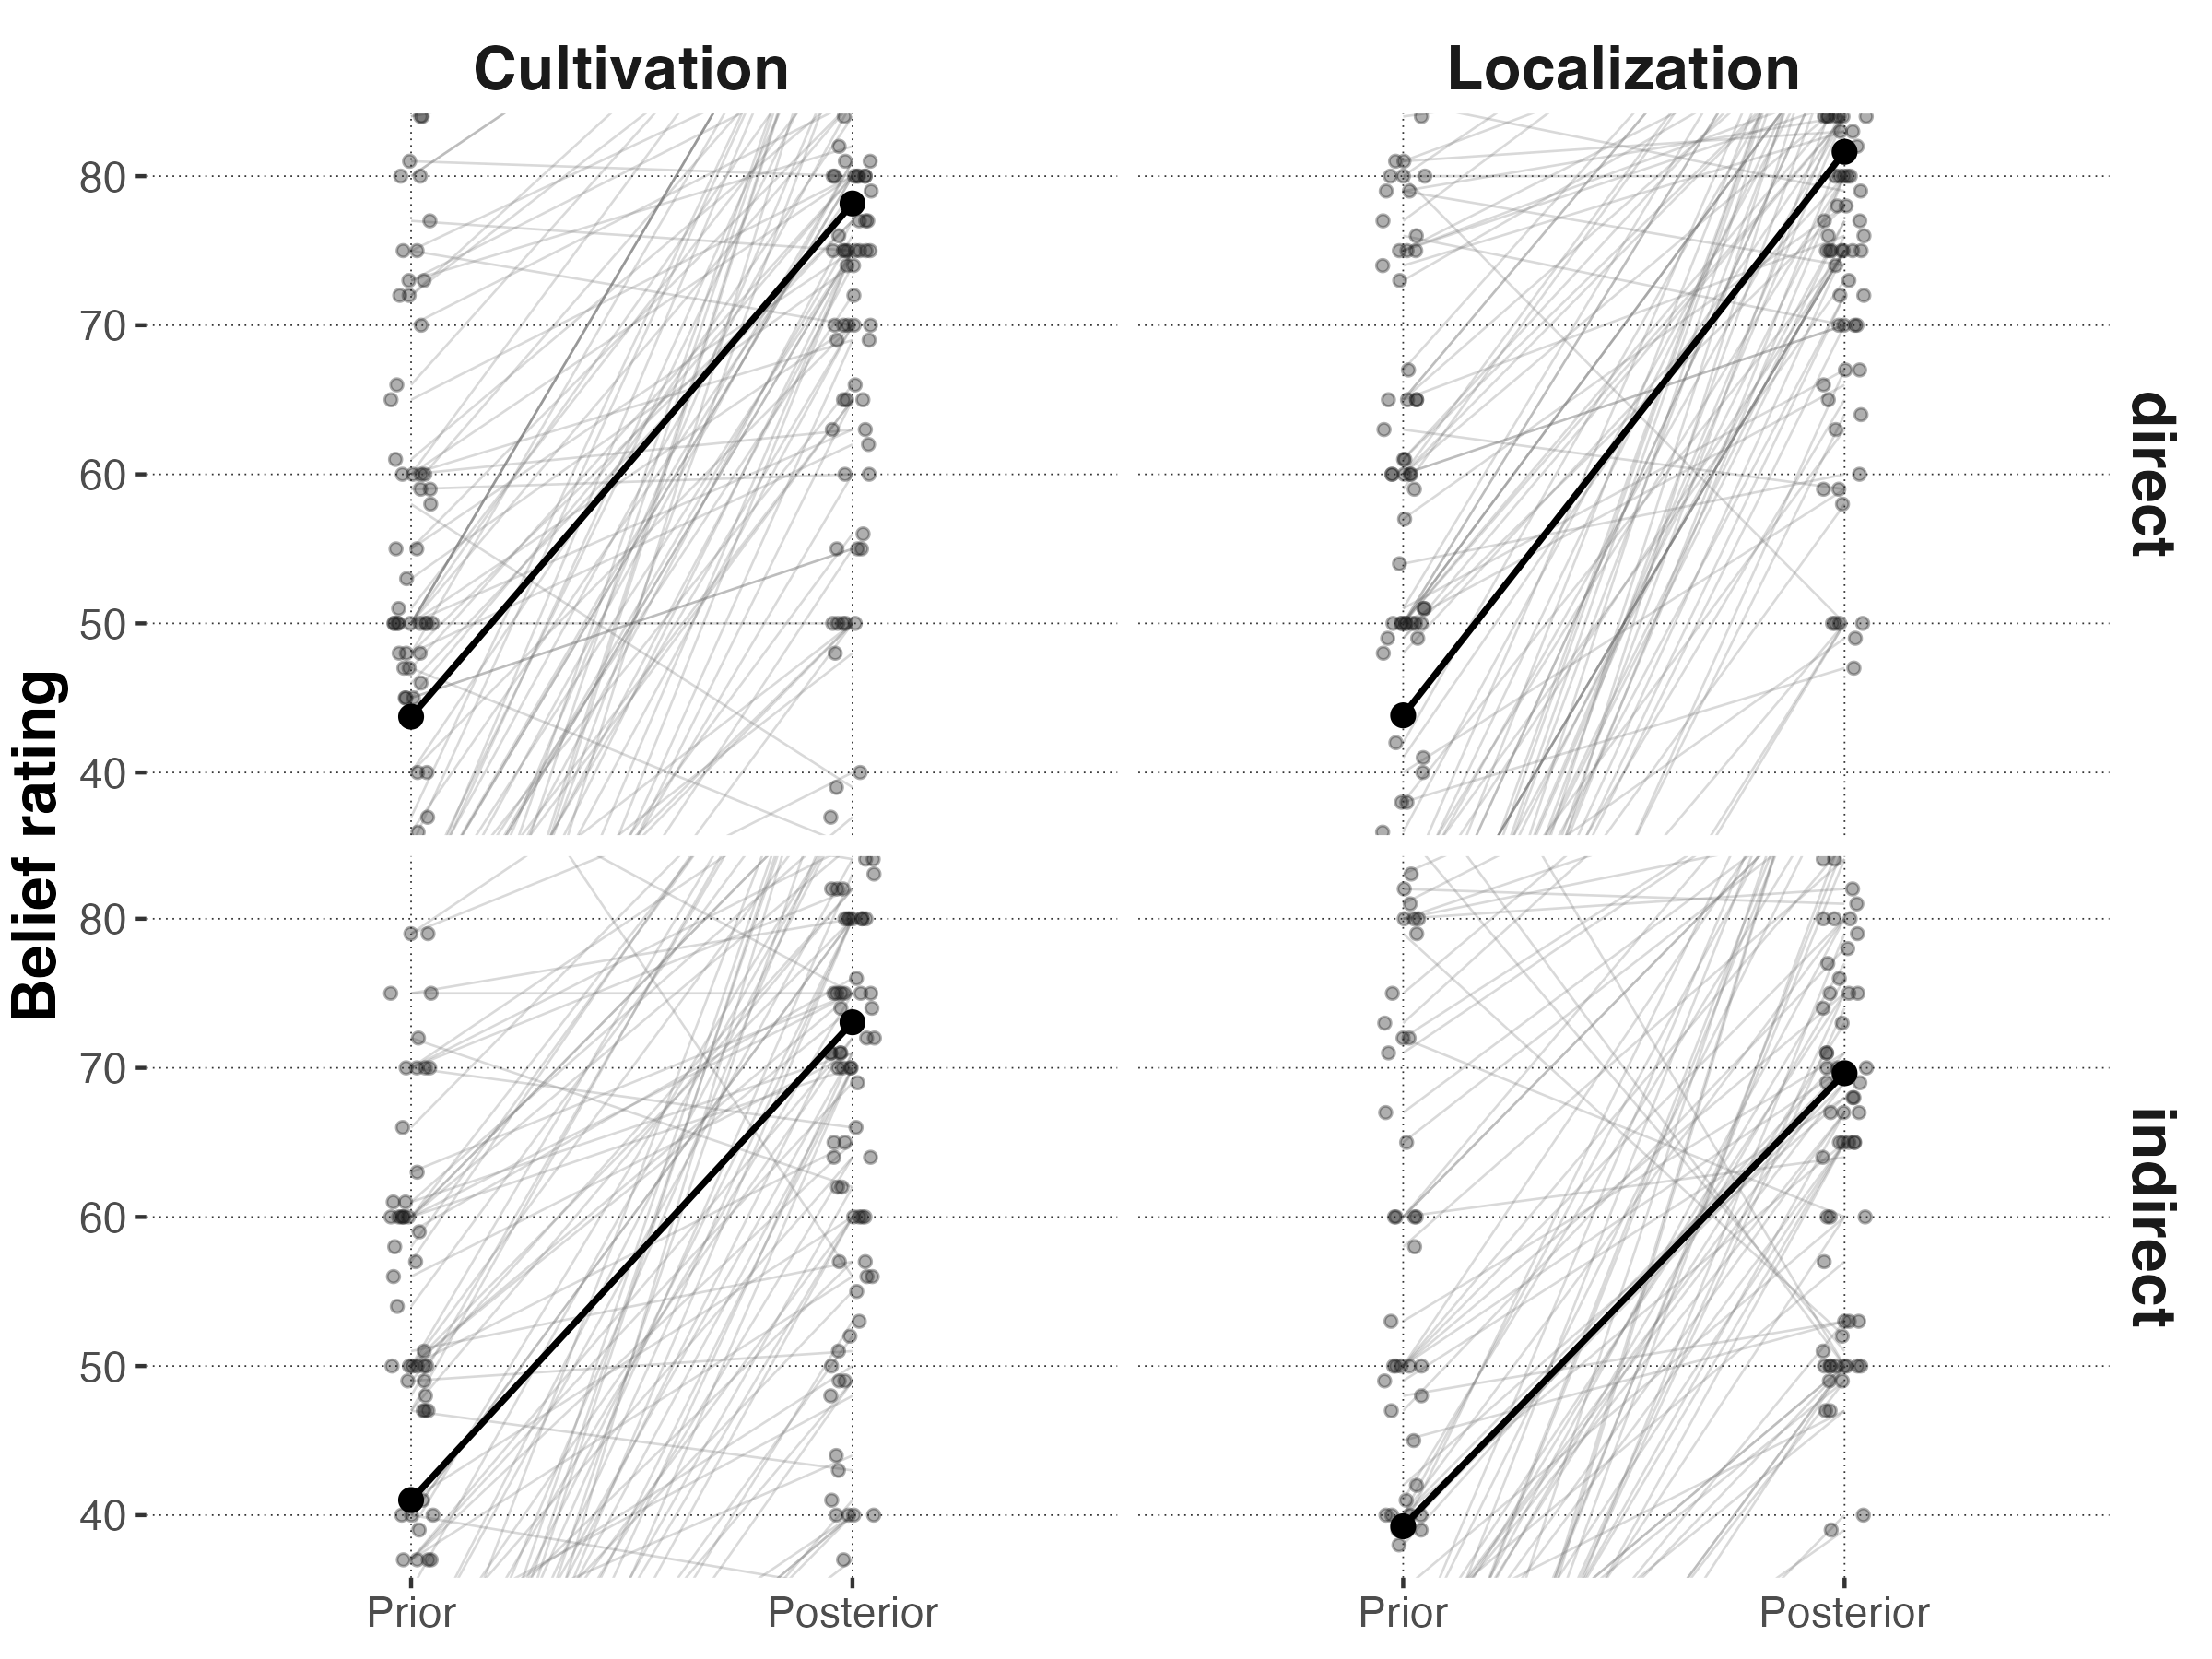
\includegraphics[width=0.99\linewidth]{figures-exp3/slope_plot.png}
%     \caption{
% slope plot}
%     \label{fig:exp2_result}
% \end{figure}


% \begin{figure}[h!]
%     \centering
%     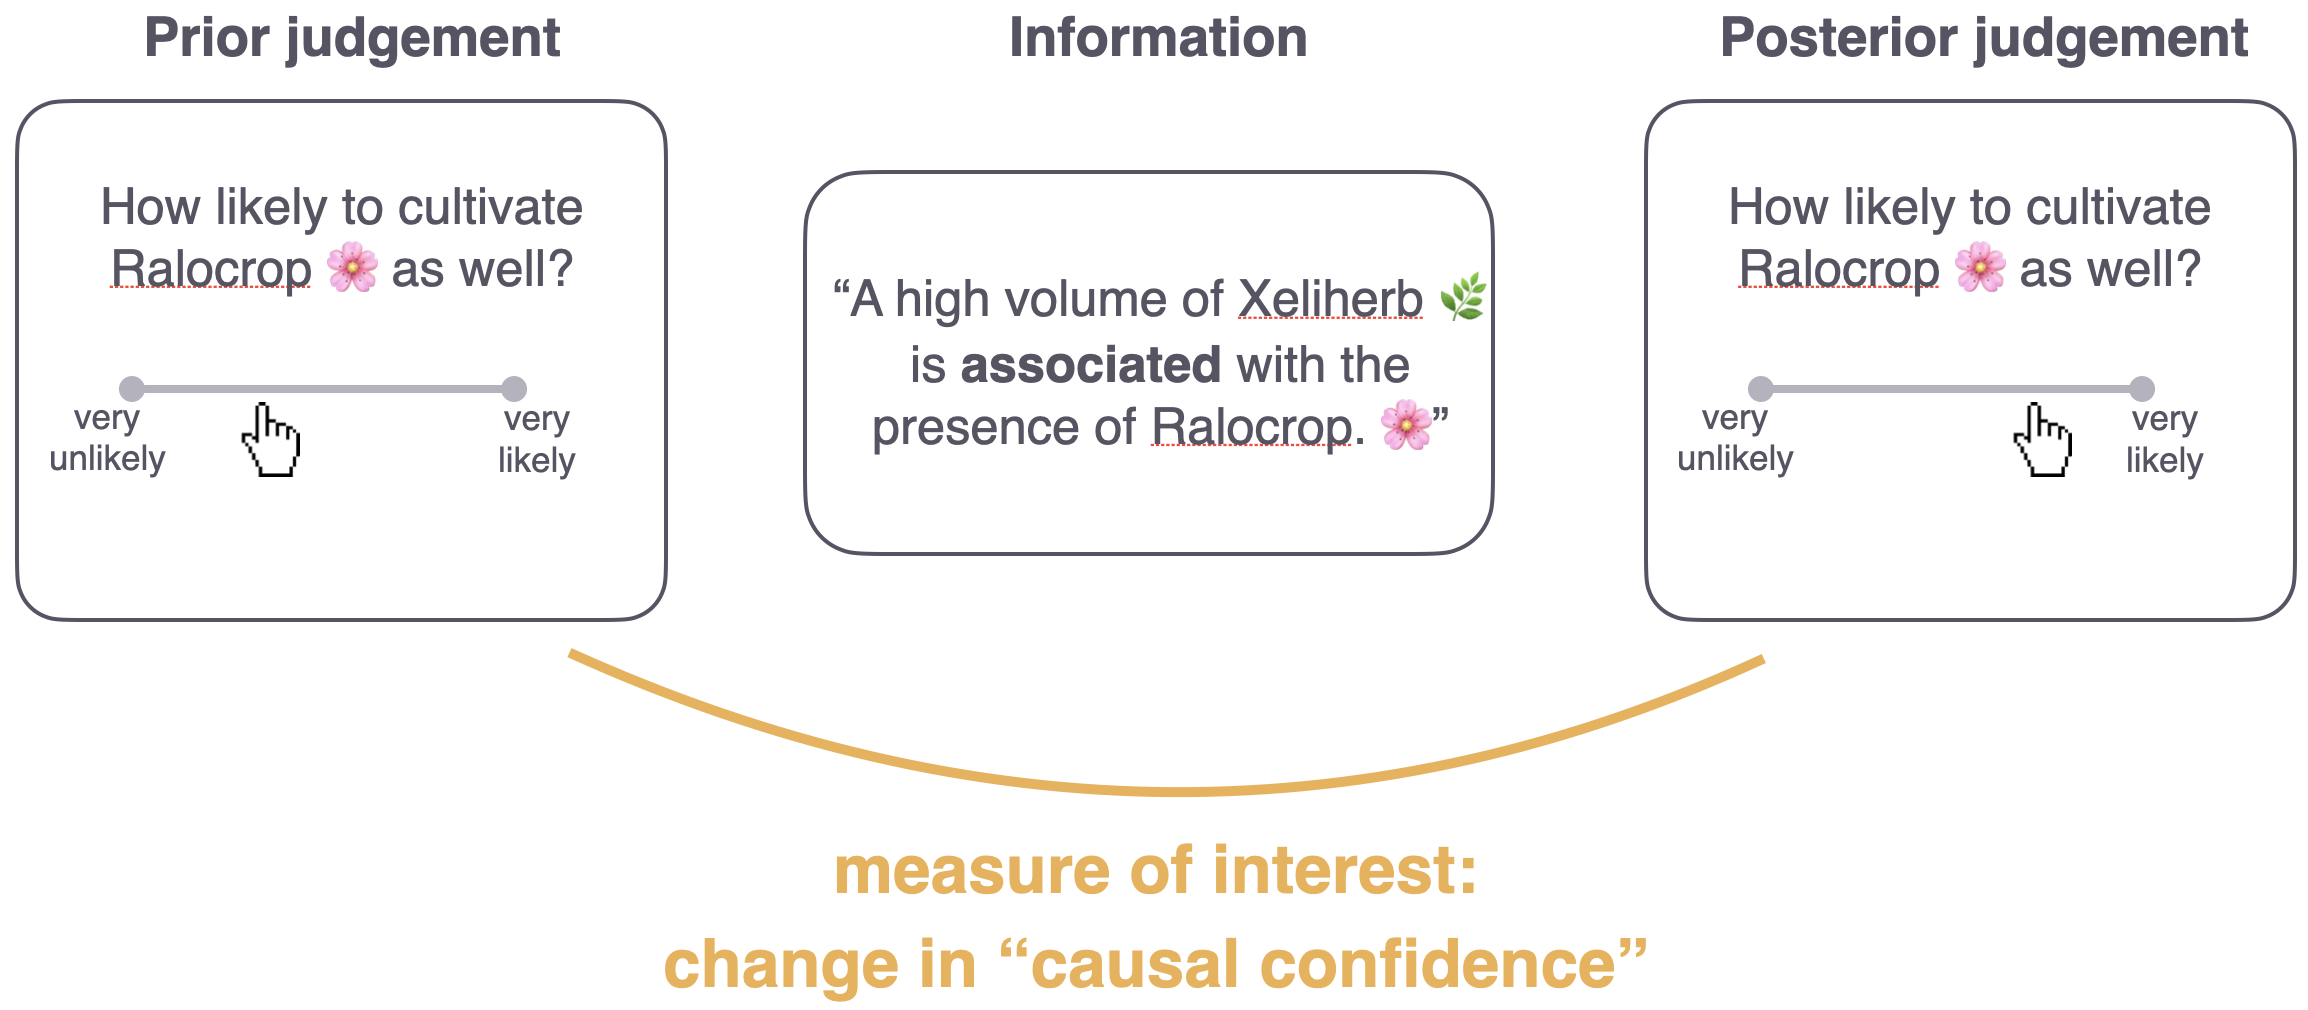
\includegraphics[width=0.9\linewidth]{figures-exp3/illustration_update.png}
%     \caption{Illustration of the procedure in Experiment~2. Participants first provided a prior judgment of how likely they would cultivate \textit{Ralocrop}. After receiving correlational information relating \textit{Ralocrop} to \textit{Xeliherb}, they provided a posterior judgment using the same scale. The change between the two judgments serves as a measure of causal belief updating.}
%     \label{fig:exp2_updateillustration}
% \end{figure}


\begin{figure}[t!]
    \centering
    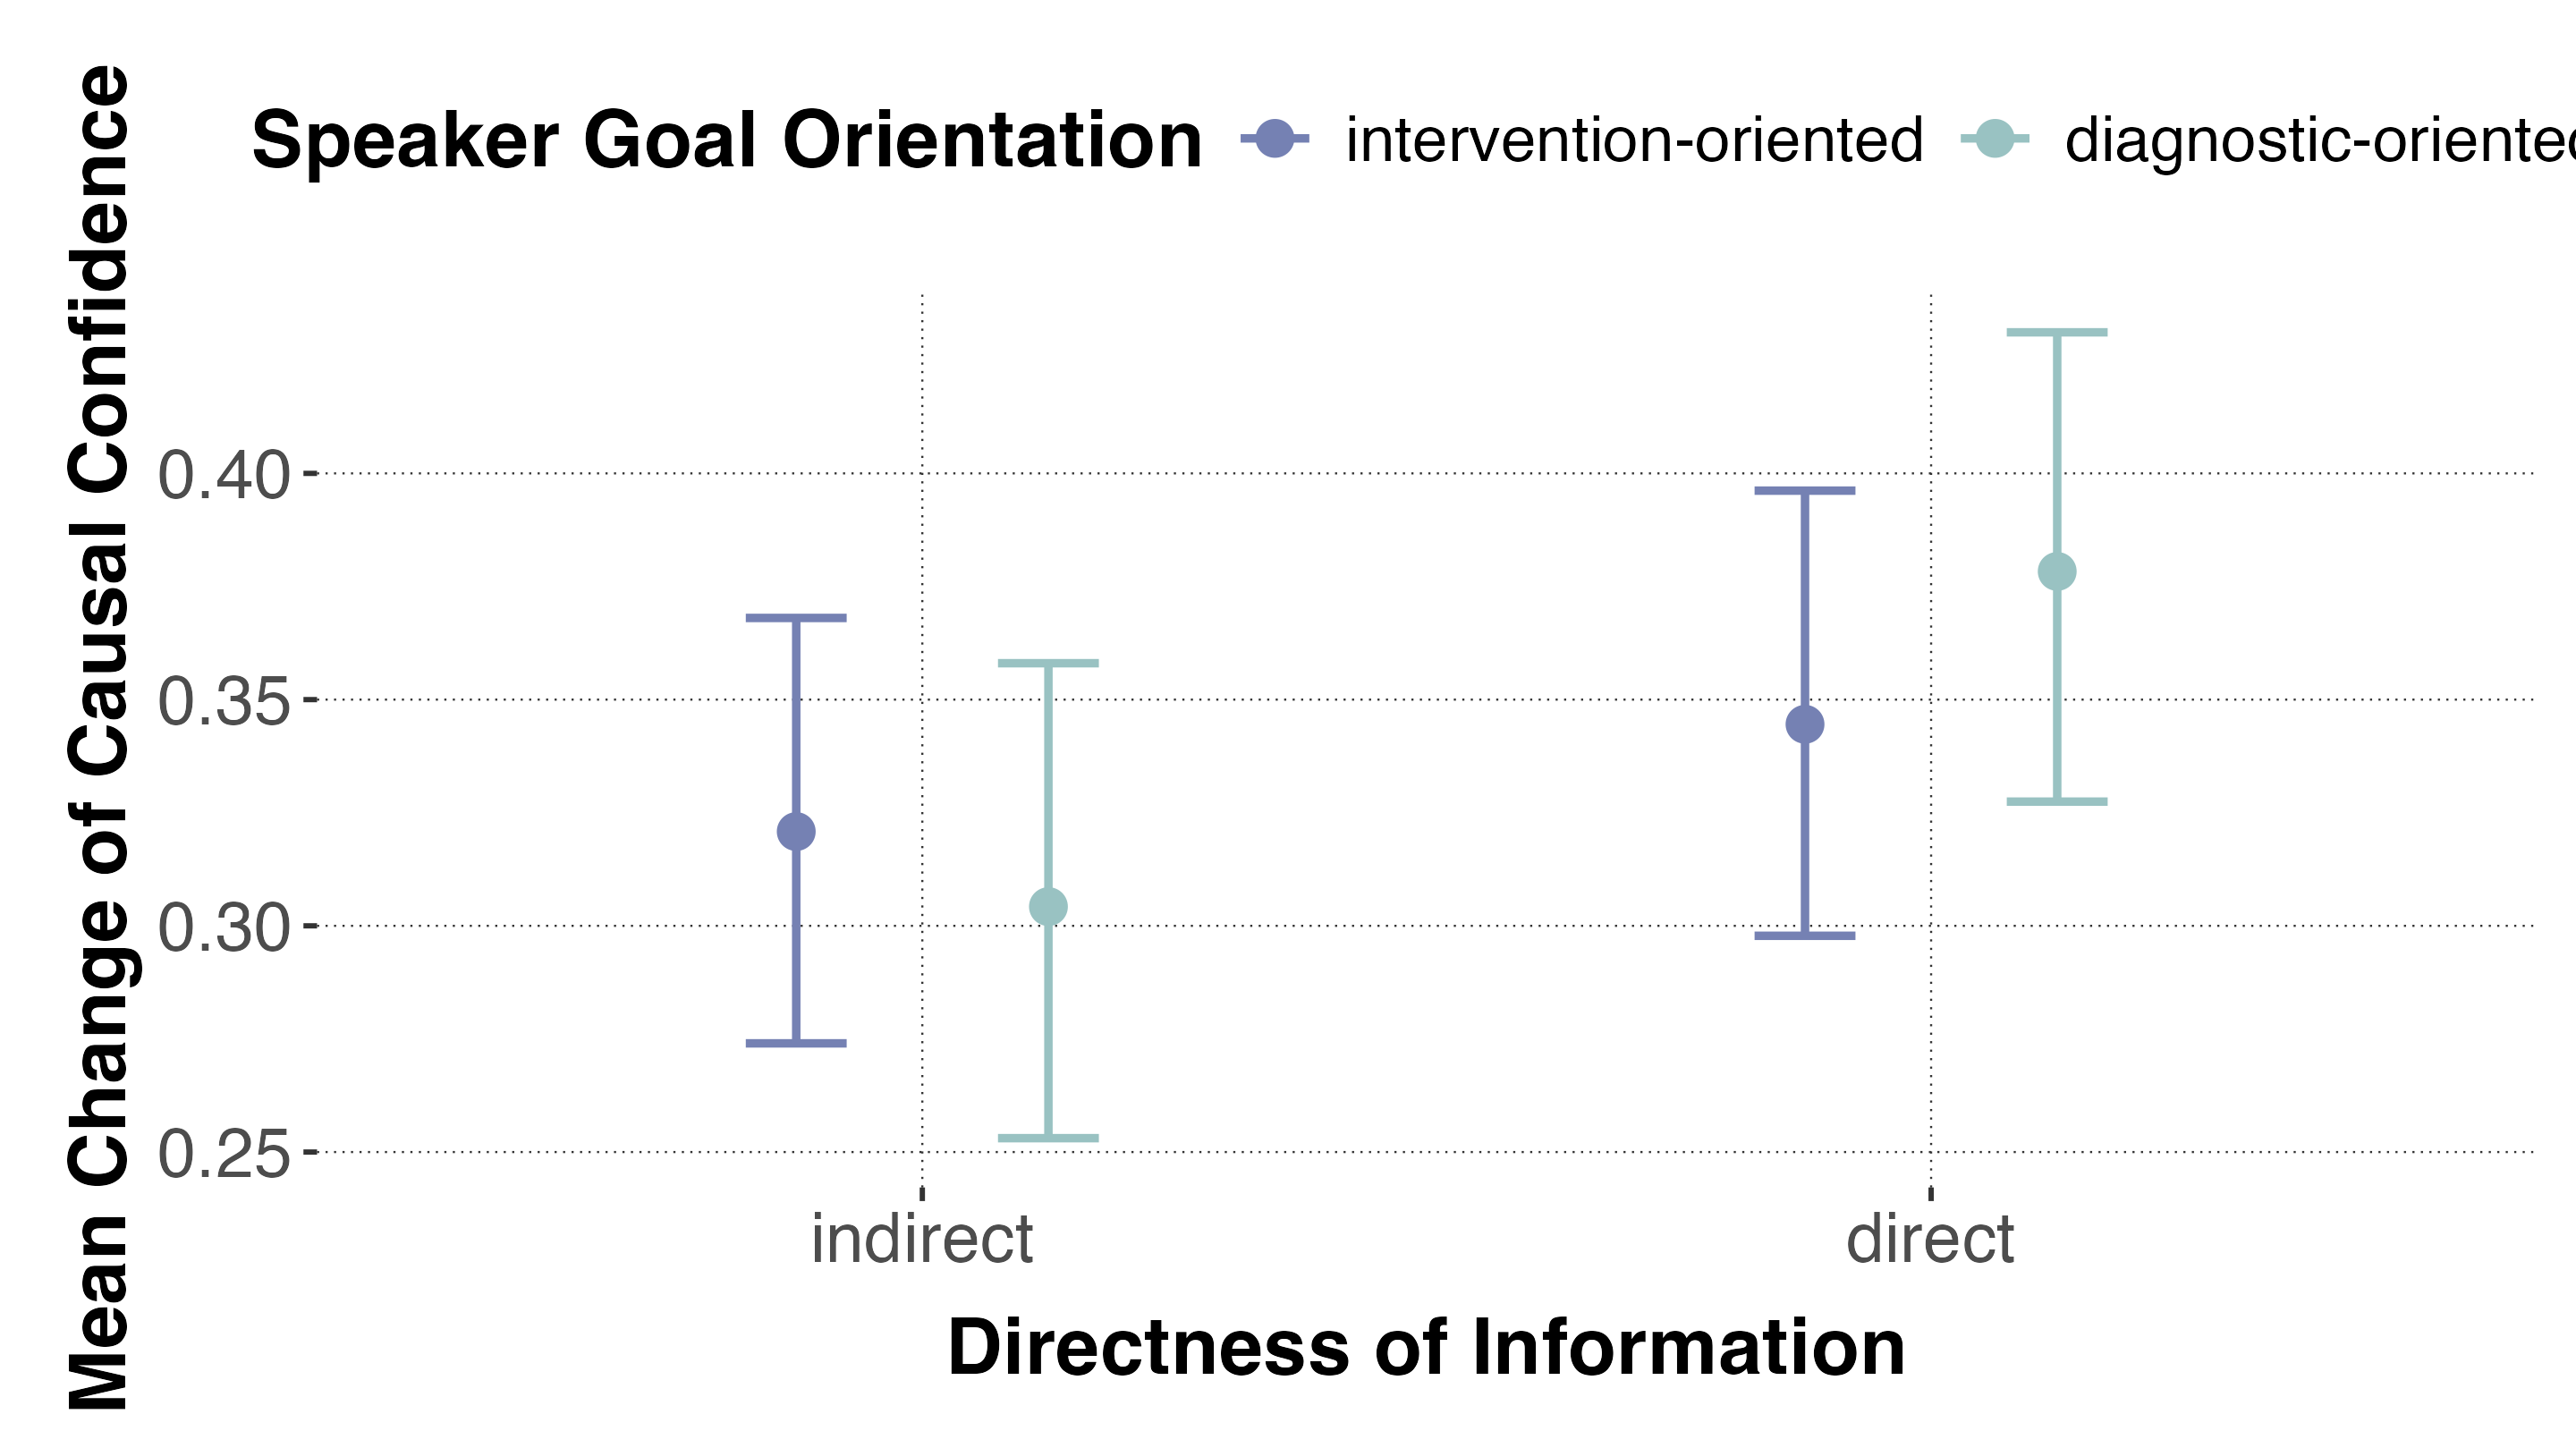
\includegraphics[width=\linewidth]{figures-exp3/results_exp_3.png}
    \caption{
Mean change in causal confidence (posterior minus prior ratings) aggregated over raw participant responses and across conditions. Points represent condition means; error bars indicate bootstrapped 95\% confidence intervals.
%\mf{I removed the "sliders from 0 to 100" part for compactness; can we please redo this plot once more with y-axis labels for the unit interval (all number / 100), please?}
}
    \label{fig:exp2_result}
\end{figure}

\subsubsection{Results}



Figure~\ref{fig:exp2_result} summarizes the results of Experiment~2. Data were analyzed using Bayesian hierarchical regression within the same general modeling framework as Experiment~1. 
The plot suggests that, for all conditions, difference scores (between posterior and prior judgments) are positive on average, indicating that the received correlational information made participants endorse an action which is rational for a belief in causation more.
The plot also suggests a possible main effect of factor \textsc{information source}, no main effect of \textsc{speaker goal orientation}, but possibly a credible interaction between these factors.

Because participants provided two judgments using a continuous slider and showed substantial heterogeneity in how they used the scale, we modeled responses as a function of \textsc{decision order} (prior vs.\ posterior judgment), \textsc{information source}, \textsc{speaker goal orientation}, and their interaction. By design, the experimental factors affected only the posterior judgment, while the prior judgment served as an individually measured baseline. The model also included by-participant random intercepts and random slopes for \textsc{decision order}, allowing baseline beliefs and belief updating to vary across individuals. To account for the bounded and non-Gaussian nature of the slider responses, slider judgments were mapped on the unit interval and modeled using a zero--one--inflated Beta likelihood. This approach allows graded belief states to be captured by the Beta component while treating exact boundary responses (0 and 1) as categorical commitments.  

The model revealed substantial individual differences in both baseline beliefs and belief updating, with participants varying widely despite identical initial conditions. The response distribution showed a clear distinction between graded belief updates and categorical commitments, with most extreme responses leaning toward the upper bound—indicating full commitment to a causal interpretation.

% \paragraph{Random effects and distributional components.}
% The hierarchical model revealed substantial individual differences in both baseline beliefs and belief updating. Participant-level intercepts showed large variability ($\sigma = 0.97$, 95\% CrI $[0.81, 1.13]$), indicating heterogeneous baseline beliefs at the first decision point despite identical slider initialization, and random slopes for decision time were also substantial ($\sigma = 0.48$, 95\% CrI $[0.25, 0.77]$), reflecting meaningful heterogeneity in belief updating. Intercepts and slopes were strongly negatively correlated ($\rho = -0.82$, 95\% CrI $[-0.99, -0.63]$), such that participants with higher initial beliefs tended to update less, consistent with ceiling effects or regression to the mean. At the distributional level, the zero--one--inflated Beta likelihood distinguished graded belief from categorical commitment: graded responses were moderately concentrated ($\phi = 7.26$, 95\% CrI $[5.76, 9.71]$), approximately 9\% of responses were exact boundary values ($\textit{zoi} = 0.09$, 95\% CrI $[0.07, 0.11]$), and boundary responses were overwhelmingly driven to the full causal commitment rather than rejection ($\textit{coi} = 0.97$, 95\% CrI $[0.92, 1.00]$).

Fixed effects were estimated on the logit scale, but we report results in terms of posterior expected predictions on the response scale for interpretability (mapped to the 0–1 range corresponding to the 0–100 slider). %The intercept was estimated at $0.44$ (95\% CrI $[0.41, 0.47]$), corresponding to the expected graded belief at the prior decision point in the reference condition (indirect information, intervention-oriented speaker).
There was a strong positive effect of decision order ($\beta = 0.31$, 95\% CrI $[0.28, 0.34]$), indicating a substantial increase in belief from the prior to the posterior judgment, consistent with systematic belief updating following exposure to the correlational information.

Crucially, the analysis revealed a credible interaction between \textsc{directness of information} and \textsc{speaker goal orientation} ($\Delta = 0.07$, 95\% CrI $[0.00, 0.13]$, posterior probability $P(\Delta > 0) = .97$, evidence ratio = 36.38). Decomposing this interaction revealed a systematic difference in directional tendencies across levels of \textsc{directness of information}. Under direct communication, posterior beliefs tended to be higher for diagnostic-oriented than for intervention-oriented speakers ($\mu = 0.03$, 95\% CrI $[0.01, 0.08]$, $P(\mu > 0) = .94$), indicating marginal evidence for this contrast. Under indirect communication, the pattern was reversed, with posterior beliefs tending to be higher for intervention-oriented than for diagnostic-oriented speakers ($\mu = -0.02$, 95\% CrI $[-0.07, 0.02]$), with moderate evidence in this direction ($P(\mu < 0) = .88$).

In addition, there was strong evidence for a main effect of \textsc{directness of information}, with higher posterior beliefs under direct than indirect communication ($\mu = 0.06$, 95\% CrI $[0.02, 0.09]$, $P(\mu > 0) > .99$). No credible main effect of \textsc{speaker goal orientation} was observed in isolation.

\subsubsection{Discussion}

Experiment~2 provides direct evidence that correlational statements can increase participants’ willingness to intervene, indicating a genuine shift in belief in causality. Crucially, while a generic increase in belief in \textit{some} causal relation is explained by assuming that participants (implicitly) applied Reichenbach's principle of \textit{no correlation without causation}, the data suggest that participant's causal belief changed towards a more specific causal interpretation (that \textit{ralocrop} cultivation influences yield of \textit{xeliherb)}.
Moreover, the experiment suggests that changes in causal beliefs were systematically modulated by pragmatic features of the communicative context. 
In particular, belief updates were larger under direct communication—when information was explicitly addressed to the participant—than under indirect exposure. This main effect suggests that listeners are sensitive to audience design and to the inferential pressures associated with communicative intent.

When correlational information is presented as having been formulated to support a listener’s decision, it is reasonable for listeners to assume that the speaker has selected information that is generally relevant \citep{SperberWilson1995}, and in particular relevant for practical decision making \citep{BenzvanRooijOptimalAssertions2007}. 
As a result, listeners may enrich correlational statements with causal meaning in order to render them useful for action. By contrast, when the same information is encountered as impersonal or self-directed—such as a report or note not tailored to a specific decision problem—the pragmatic pressure to infer causal structure is weaker. In these cases, correlational statements can be interpreted as merely descriptive, and belief updating is correspondingly reduced.

Beyond this main effect, the interaction between communicative directness and speaker goal orientation further supports the pragmatic enrichment view by revealing not only when causal belief updating is strengthened, but also when it is attenuated.
Under direct communication, correlational statements attributed to diagnostic-oriented speakers elicited larger belief updates than those attributed to intervention-oriented speakers. This asymmetry is consistent with pragmatic reasoning over alternative utterances. When a speaker whose role already presupposes intervention nevertheless opts for a weak correlational formulation, listeners may reason more cautiously: had the speaker been confident in a causal relationship, a stronger or more directive formulation would have been communicatively preferable. This inference may block causal enrichment and attenuates belief updating.

By contrast, when a diagnostic-oriented speaker—whose own task does not presuppose intervention—directly communicates correlational information to a listener who is known to care about acting, the choice to mention a manipulable factor can be interpreted as intentional and action-relevant. Despite the lack of goal alignment, listeners may reason that the speaker selected this information precisely because it bears on the listener’s decision problem. Under this interpretation, the correlational formulation invites pragmatic enrichment: it is treated as conveying information about a causally actionable relationship, even without explicit causal language.

In indirect contexts, where the same information is encountered as impersonal evidence rather than as communicative input, opportunities for pragmatic reasoning are substantially reduced. In the absence of clear audience design, listeners have less reason to consider alternative utterances or to infer speaker intentions, and belief updating correspondingly becomes less sensitive to speaker goal orientation. Nevertheless, we observe moderate evidence for a small tendency in the opposite direction: when the information originates from an intervention-oriented context, belief updating is slightly higher, maybe reflecting alignment between the inferred function of the information and the listener’s own decision goals.

\begin{comment}
    

\section{General Discussion}

Across two experiments, we examined whether correlational language can strengthen causal beliefs in decision-making contexts, how such interpretations are mentally represented, and how pragmatic features of communication modulate these effects. Together, the results provide converging evidence that correlational statements can support causal interpretations that guide both decisions and communication.

Experiment~1 addressed the representational consequences of causal interpretation. Using recall and advice tasks, we found that participants who chose to intervene were more likely to reproduce correlational statements as explicitly causal and, in the advice task, to recommend intervention on the putative cause. Participants who did not intervene predominantly reproduced the original association or omitted relational content. These patterns suggest that intervention choices are associated with richer causal representations that are available for downstream communicative use, rather than reflecting a purely response-level bias.

Experiment~2 complemented these findings by introducing a belief-update paradigm that directly tracks changes in causal confidence within individuals. Exposure to correlational information reliably increased willingness to intervene relative to an individually measured baseline, providing direct evidence that correlational language can strengthen causal belief. Crucially, belief updating depended on pragmatic features of the communicative context: differences between diagnostic-oriented and intervention-oriented speakers emerged only under direct communication, where listeners could plausibly reason about speaker intent. When the same information was encountered through an impersonal source, these contrasts disappeared.

Taken together, these findings support a pragmatic account of causal interpretation in which listeners enrich correlational statements by reasoning about speakers’ goals and communicative choices, particularly in contexts where action is at stake. \DL{See comment in Overleaf - I think the explanation of what the exp2 results mean could be improved.}
\end{comment}
\section{Conclusion}

The present study revisits a tension in causal reasoning: although correlational statements are semantically compatible with multiple causal structures, listeners often enrich these statements to carry more specific causal information. Across two experiments, we show that correlational language can strengthen causal beliefs in decision-making contexts, that such beliefs are reflected in both own interpretations and action-guiding communication, and that pragmatic properties of the communicative context systematically modulate when causal enrichment is strengthened or attenuated. 
These findings are difficult to capture with accounts that relate causal enrichments to a simple bias or heuristic, but follow naturally from a pragmatic account in which causal implicatures arise through reasoning about the communicative context.

%Experiment~1 provides evidence that causal interpretations of correlational statements are reflected not only in participants’ immediate judgments, but also in their internalized interpretations and in how they communicate information to others. Across both recall and advice tasks, participants who chose to act on the putative cause were more likely to reproduce the correlational statement using explicitly causal language than participants who did not intervene. This pattern was especially pronounced in the advice task, where participants were required to tailor information for another agent. In this sense, Experiment~1 illustrates a mechanism by which causal enrichment from correlational language can be externalized and propagated through communication.

The finding that speakers are more likely to use causal language when advising others (Experiment~1), and that listeners are more likely to draw causal inferences when the information is communicated directly (Experiment~2), mirrors everyday patterns of word-of-mouth and social-media communication. In such contexts, correlational findings are often encountered directly and then passed on as recommendations or advice. When individuals choose to act on this information, they may reframe it in causal terms for others, thereby amplifying its apparent causal force through successive message passing. Crucially, this transformation does not require intentional distortion; instead, it can arise naturally from pragmatic reasoning about what information is most relevant or useful for another person’s decision-making context.

%Experiment~1 demonstrates how such enrichment can emerge even when the original message is explicitly correlational under communicative settings.

%Experiment~2 complements these findings by directly measuring belief updating within individuals in a decision-relevant context. Using a belief-update paradigm based on willingness to intervene, we show that exposure to correlational information reliably increases causal confidence relative to an individually measured baseline. Crucially, this updating is systematically modulated by pragmatic features of the communicative context. Direct communication—where information is explicitly addressed to a listener—produces stronger belief updates than indirect exposure. Moreover, speaker goal orientation interacts with directness: under direct communication, correlational statements from diagnostic-oriented speakers elicit larger belief updates than those from intervention-oriented speakers, whereas this contrast is attenuated under indirect exposure. Together, these results identify not only the conditions under which causal belief updating is strengthened, but also those under which it is selectively reduced, in a manner consistent with pragmatic reasoning about communicative intent and alternative utterances.

%Taken together, the two experiments provide converging evidence for a pragmatic account of causal implicature. Experiment~1 shows how causal interpretations are represented and communicated, while Experiment~2 demonstrates how those interpretations translate into graded belief updating under varying pragmatic factors. The combined results suggest that listeners enrich correlational language with causal meaning by reasoning about why a speaker chose a particular formulation given their goals and the communicative setting, rather than by mechanically over-attributing causation.

Several limitations remain. First, while the current paradigm captures decision-making behavior in response to correlational information, it does not fully disentangle causal belief from utility-based reasoning. Future work could address this by separately modeling inferred causal structure and subjective cost–benefit considerations. Second, our experiments focused primarily on pragmatic cues related to speaker goals and communicative framing; exploring how inferences are shaped by the listener’s own goals and relevance constraints would offer a valuable extension. Finally, formalizing the observed effects within probabilistic pragmatic frameworks \citep{goodman2016pragmatic,ScontrasTessler2021:A-practical-int,Degen2023:The-Rational-Sp}, in particular extending previous like-minded models of causal enrichments of conditionals \citep{grusdt_probabilistic_2022}, could yield more precise, model-based predictions about when and how causal enrichment arises from correlational language.


% \section{Acknowledgments}

% Some illustrative images used in Experiment~2 were generated with the assistance of AI-based image generation tools (ChatGPT) and were used solely for visualization and contextual support; they did not affect the experimental logic or data analysis.

\printbibliography

\end{document}
